\documentclass[12pt,a4paper]{article}

\usepackage{amsmath,amsfonts,amssymb}
\usepackage{graphicx}
\usepackage{geometry}
\usepackage{hyperref}
\usepackage{booktabs}
\usepackage{algorithm}
\usepackage[noend]{algpseudocode}
\usepackage{mathptmx}

\algrenewcommand\algorithmicrequire{\textbf{Input:}}
\algrenewcommand\algorithmicensure{\textbf{Output:}}
\algrenewcommand\algorithmicif{\textbf{If}}
\algrenewcommand\algorithmicthen{\textbf{Then}}
\algrenewcommand\algorithmicelse{\textbf{Else}}

\graphicspath{{../figures/}}

\geometry{left=2.5cm,right=2.5cm,top=2.5cm,bottom=2.5cm}
\renewcommand{\topfraction}{0.9}
\renewcommand{\bottomfraction}{0.8}
\renewcommand{\textfraction}{0.08}
\renewcommand{\floatpagefraction}{0.82}
\setcounter{topnumber}{3}
\setcounter{bottomnumber}{2}
\setcounter{totalnumber}{4}

\title{\textbf{Signed-Distance-Field Local Geometry Feedforward for Complementarity-Based Rigid-Body Contact}}
\author{
    Lijing Wang$^1$, Wei Fan$^2$, Hui Ren$^{1,2,*}$\\[1em]
    $^1$Faculty of Computing, Harbin Institute of Technology, Harbin, China\\
    $^2$Institute of Aerospace Vehicle Dynamics and Control,\\
    School of Astronautics, Harbin Institute of Technology, Harbin, China\\[0.5em]
    $^*$Corresponding author: renhui@hit.edu.cn
}
\date{}

\begin{document}

\maketitle

\begin{abstract}
Signed-distance-field local geometry feedforward provides a low-intrusion way to improve complementarity-based rigid-body contact without rewriting the underlying solution chain. This paper presents a complementarity-based rigid-contact model built around that idea. Within a Moreau--Jean framework, local geometric information from a signed distance field is used to construct regime-dependent contact representations. Smooth continuously evolving contact is treated with a persistent-manifold SlidingPatch representation augmented by Hessian-based curvature feedforward, whereas contact onset, compact contact zones, and switching-sensitive cases are handled with a more conservative CompactDiscrete representation. The geometric correction is introduced only through a feedforward modification of the effective normal gap, so the underlying linear complementarity problem (LCP) solution chain is preserved.

Results from head-on impact, an eccentric disk--roller analytical benchmark, the Onset Stress Benchmark, an industrial cam, and a Twin Gear case show that regime-matched local-geometry-aware modeling improves gap prediction and reduces trajectory and velocity errors while keeping the additional modeling overhead controlled. The gain is most evident in sustained-sliding and contact-onset scenarios. Near singular boundaries or under nonsmooth meshing, more conservative discrete representations provide better robustness. The benchmarks support two conclusions: the full local-geometry-aware modeling stack is effective within a complementarity-based rigid-contact framework, and curvature feedforward yields additional gains when the underlying local manifold remains smooth. Overall, the proposed method is a regime-matched modeling strategy that improves contact-response accuracy without sacrificing computational efficiency under clearly stated applicability conditions.

\end{abstract}
\noindent\textbf{Keywords:} rigid-body contact; linear complementarity problem; signed distance field; local geometric representation; nonsmooth multibody dynamics

\section{Introduction}
Signed-distance-field local geometry feedforward offers a low-intrusion way to strengthen complementarity-based rigid-body contact. Nonsmooth contact dynamics based on velocity-level time-stepping schemes and linear complementarity problems (LCPs) remains one of the core paradigms for rigid-body collision, intermittent contact, and contact-state transitions in robotics simulation, computer graphics, and engineering multibody dynamics \cite{flores2022contact,wang2021nonsmooth,stewart1996implicit,anitescu1997formulating}. Within this class of methods, complementarity constraints provide a natural way to impose non-penetration, impact response, and contact-state switching, which is why they remain particularly attractive for intermittent rigid contact. Practical contact quality, however, is determined not only by the algebraic form of the constraints but also by how local geometric information enters the model.

Conventional contact detection usually relies on polygon meshes and boundary-distance queries, with GJK and its descendants serving as representative examples \cite{gilbert1988fast,wang2021collision}. In recent years, the emergence of sparse voxel storage, GPU-friendly data structures, and SDF-based collision handling has made the use of signed distance fields (SDFs) as implicit surrogates for rigid-body surfaces increasingly attractive \cite{museth2021nanovdb,macklin2020sdfcollision,liu2024sdfsdf,lai2024unifying,lopez2024convexsdf}. However, within a complementarity-based rigid-contact framework, if local geometry enters only through the distance value $\Phi$ and the first-order gradient $\nabla \Phi$, the contact normal, gap evolution, and constraint response can become highly sensitive to local geometric error during contact onset, sustained sliding, and local state transitions. In geometrically demanding scenarios such as cam tips, roller transition zones, and gear boundaries, this sensitivity may manifest itself as velocity spikes, peak errors, and degraded tracking behavior.

In this setting, the focus of the present work is not the redesign of the underlying complementarity solver, but the input-layer modeling problem that arises when SDF geometry is coupled to an existing solver chain. In many engineering cases, the limiting factor is whether local geometric information enters the contact model in a sufficiently stable and accurate manner, especially in the prediction of gap evolution, the description of local normal manifolds, and the control of geometric noise during contact activation. From this perspective, a low-intrusion enhancement of the geometry-to-solver interface within an established LCP framework is more aligned with the problem structure addressed here than the construction of yet another rigid-contact solver.

It is important to stress that the present work does not attempt to extend complementarity-based methods into regimes that are better handled by penalty-based formulations, such as soft contact or complex distributed contact. Instead, the focus is a more basic modeling question within the valid scope of complementarity-based rigid contact: \textbf{without changing the existing hard-contact complementarity solution framework and without switching to penalty-based soft-contact modeling, how should local contact geometry be represented so that more accurate contact responses can be obtained during contact onset, sustained contact, and state transitions without sacrificing computational efficiency?} In other words, the question is not whether one enhanced geometric proxy can universally outperform traditional approaches, but rather how local geometric information should enter a complementarity-based rigid-contact model in a way that matches the contact state and converts geometric detail into simultaneous gains in numerical accuracy and computational efficiency under clearly defined applicability conditions.

To address this question, this paper develops a \textbf{local-geometry-aware complementarity-based rigid-contact modeling strategy}. Within a unified Moreau--Jean time-stepping framework, local geometric information from the SDF is used to construct local representations in the neighborhood of contact, and the representation is configured according to the contact state. For cases with continuous local contact evolution and relatively smooth sliding, a \texttt{SlidingPatch} representation with a persistent manifold is adopted, and Hessian-based curvature feedforward is injected on the corresponding local manifold. For cases characterized by contact onset, compact local contact domains, or sensitivity to state transitions, a more compact and conservative \texttt{CompactDiscrete} representation is used to preserve numerical robustness. In the current implementation, this selection is performed through case- or application-level preset configuration rather than runtime switching by a unified classifier. Accordingly, the main purpose of this work is neither to replace the underlying solver nor to propose an automatic regime-identification algorithm, but to analyze whether regime-matched local geometric representations can improve numerical accuracy without sacrificing computational efficiency inside an existing complementarity-based rigid-contact framework.

The main contributions of this work are as follows:
\begin{itemize}
    \item \textbf{A local-geometry-aware complementarity model for rigid contact.} Local SDF-based geometric information is introduced at the contact-modeling level without replacing the mature global solver backbone. This places the improvement explicitly at the geometry-to-solver interface, enriches the geometric description near the contact region, and supports accurate contact simulation without sacrificing computational efficiency within the intended application regimes.
    \item \textbf{A contact-state-oriented configuration strategy for local representations.} For continuous sliding, a continuous \texttt{SlidingPatch} representation is combined with local curvature feedforward; for contact onset, compact contact domains, and state-transition-sensitive cases, a compact discrete \texttt{CompactDiscrete} representation is adopted, so that the use of local geometry is grounded in a representation matched to the contact regime.
    \item \textbf{A systematic validation of the applicability of local-geometry-aware modeling using existing benchmark cases.} Through head-on impact, an eccentric disk--roller analytical benchmark, the Onset Stress Benchmark, an industrial cam, and a Twin Gear case, the proposed modeling strategy is evaluated across different contact scenarios. The results show that, under regime-matched settings, it improves local geometric description and global numerical response in continuous sliding and contact-onset problems while maintaining computational efficiency; in the presence of local singular boundaries or nonsmooth meshing/contact transitions, its effectiveness depends more strongly on the match between local representation and contact state.
\end{itemize}

It should also be emphasized that the experiments in this paper are not intended to prove that one single regime is universally optimal across all benchmarks. Instead, each benchmark is regarded as a representative scenario associated with a particular contact state, and the proposed modeling strategy is assessed under a preconfigured regime matched to its local geometric characteristics so as to examine whether stable, interpretable, and practically meaningful gains in both efficiency and accuracy can be obtained. The ultimate outcome is therefore a modeling principle for regime-matched contact simulation rather than a runtime algorithm that automatically selects the best local representation.


\section{Related Work}
\subsection{Nonsmooth contact and multibody time-stepping}
Classical rigid-contact solvers can be broadly divided into two lines: penalty/compliant contact and nonsmooth contact based on complementarity or differential variational inequalities. Jean's nonsmooth contact dynamics, the Stewart--Trinkle implicit time-stepping scheme, and the LCP/constraint-stabilization work of Anitescu--Potra and Anitescu--Hart collectively established the modern classical foundation of rigid contact based on velocity-level time stepping, unilateral constraints, and complementarity modeling \cite{jean1999nonsmooth,stewart1996implicit,anitescu1997formulating,anitescu2004constraint,anitescu2010iterative,tasora2011matrixfree,pfeiffer2012nonsmooth}. More recent tutorials and surveys have provided broader syntheses of contact constraints in Lagrangian systems, rigid-body frictional contact, and multibody contact mechanics \cite{contacttutorial2016,contactconstraints2016,flores2022contact,wang2021nonsmooth,peng2022sensitivity}.

Building on this foundation, work on specific solvers, contact patches, flexible multibody systems, quasistatic stepping, and numerical comparisons has further expanded the solution landscape of this line of research \cite{melanz2017comparison,catchingup2018,contactpatch2018,symplecticcontact2019,flexiblecontact2020,convexquasistatic2021,effectivemass2022,contactbasics2023,predictioncorrection2025,contactmultiscale2025}. On the implementation and application side, studies on flexible multibody strategies for large lap joints, rigid/compliant comparisons, wheel--rail conformal contact, automatic contact detection, and improved polygonal contact have advanced engineering usability from the perspectives of software realization, contact representation, and detection pipelines \cite{lapjoints2016,pazouki2017compliant,conformalwheel2020,autocontact2023,polygonalcontact2023,nencioni2025conformal,gradientcontact2025}. In robotics control and contact-rich manipulation, rigid contact and friction have also been incorporated explicitly into inverse dynamics and convex time-stepping formulations \cite{inversedynamics2016,convexquasistatic2021}.

It is important to emphasize that the LCP/MLCP line does not correspond exactly to ``all real contact,'' but rather to an idealized rigid-body nonsmooth contact model: bodies are treated as rigid, contact is represented by unilateral non-penetration constraints, and local elastic compression and contact-patch evolution are not resolved explicitly; instead, velocity or impulse updates satisfy complementarity conditions over discrete time steps \cite{jean1999nonsmooth,stewart1996implicit,anitescu1997formulating,contacttutorial2016,flores2022contact,wang2021nonsmooth}. As a result, this line most naturally describes constraint response, impulse transfer, and contact-state transitions in discrete time rather than the full local mechanics of contact in a continuum sense. Accordingly, LCP-based methods are most appropriate for rigid-body, multi-contact, impulse-dominated problems with frequent contact/separation switching. In near-conformal or large-area contact, local elastic compression and Hertz-type contact-patch evolution, lubrication- or adhesion-dominated contact, rate- and history-dependent friction, and cases requiring accurate contact timing, impact waveforms, or smooth local force histories, the results should be interpreted as equivalent constraint responses at the discrete-time level rather than as complete descriptions of real contact mechanics \cite{pazouki2017compliant,contactpatch2018,nencioni2025conformal}. In this sense, the literature has largely explained why complementarity-based rigid contact is meaningful, but it still lacks a systematic discussion of \emph{how local geometry should enter the contact model within this framework}.

\subsection{Implicit geometry, distance fields, and collision surrogates}
In geometry representation and collision detection, boundary-distance-based convex queries have long been shaped by GJK, Baraff's rigid-contact analysis, and dynamic BVH techniques, while cloth and deformable-body collision detection has further highlighted the importance of robust contact handling for dynamic quality \cite{gilbert1988fast,baraff1989analytical,baraff1994fast,larsson2006dbvh,bridson2002robust,teschner2005collision,wang2021collision}. On the other hand, distance fields have long served as implicit geometric surrogates for shape representation, sphere tracing, sparse voxel organization, and high-resolution narrow-band representations. ADF, sphere tracing, OpenVDB, and NanoVDB represent key developments in adaptive sampling, robust querying, and sparse data structures for distance fields \cite{frisken2000adf,hart1996sphere,museth2013vdb,museth2021nanovdb}.

For contact and collision processing based on SDFs, prior studies have investigated point-to-SDF continuous collision detection, locally optimized robust SDF collision handling, contact between beams/flexible bodies and discrete SDFs, SDF-DEM modeling for arbitrary granular shapes, SDF-enhanced CFD-DEM, real-time collision detection between general SDFs, and unified formulations bridging SDF contact and traditional discrete-element contact \cite{hapticsdf2017,macklin2020sdfcollision,sdfbeam2020,sdfdem2022,sdfcfddem2023,liu2024sdfsdf,lai2024unifying,lopez2024convexsdf}. More recent work has further discussed piecewise-continuous interpolation for SDFs, moving-SDF contact formulations, SDF-based conformal contact detection, dynamic SDF reconstruction for irregular deformable bodies, and the possibility of promoting SDFs to general proxies for robotic multi-contact \cite{adaptivesdf2023,movingframesdf2024,superellipsecontact2025,dynamicreconsdf2025,contactsdf2025}. These studies clearly demonstrate the value of SDFs as geometric surrogates, but they focus primarily on geometric queries, collision detection, compliant/proximal-style contact formulations, or generic contact proxy capability. In contrast, \emph{how local SDF geometry can improve contact modeling while preserving the main complementarity-based rigid hard-contact solution chain} remains insufficiently articulated. At the same time, interpolation, differencing, and nearest-point branch switching can amplify discontinuities in normals and curvature at the sub-voxel level, which means that the manner in which SDF geometry enters the dynamics model must itself be designed carefully.

\subsection{Local geometric representation and contact stabilization}
Computer graphics and geometric simulation have also long recognized the limitations of first-order contact approximation and have developed a variety of position-level, compliant-level, and patch-level stabilization strategies. Representative examples include Position Based Dynamics, XPBD, position-based solid simulation with improved contact accuracy, small-step explicit stabilization, and extended PBD variants for rigid bodies \cite{muller2007pbd,macklin2016xpbd,francu2017solids,macklin2019smallsteps,xpbdrigidbody2020}. Another class of work starts from asynchronous or variational contact and seeks to improve robustness and parallelism in complex contact through finer event handling or more consistent energy-based contact models \cite{harmon2009acm,vouga2011avcm,ainsley2012spacm}.

In optimization-based, proximal, and monolithic contact modeling, proximal-operator approaches, IPC, FrictionalMonolith, intersection-free rigid-body dynamics, contact-and-friction courses for graphics, monolithic frictional contact treatment for rigid/fluid systems, and recent unified handling of contact, friction, and shock propagation offer alternatives to the classical velocity-level LCP complementarity chain from the perspectives of unknowns, stabilization pathways, and coupling structure \cite{proximalcontact2017,li2020ipc,frictionalmonolith2021,contactgraphicscourse2021,intersectionfree2021,sphcontact2023,unifiedshock2023,chen2024primaldual}. In contrast to these position-level, optimization-level, or explicit proximal lines, the present work is concerned with a different question: how local geometric representation should enter the contact model without rewriting the underlying complementarity-based rigid-contact solution chain. Specifically, we do not treat the SDF as a universal contact proxy whose superiority must be established independently; rather, we use it as a carrier of local geometric information to construct patch-level local representations, generate curvature feedforward, and adopt different local modeling modes under preconfigured regimes corresponding to different contact states.


\section{Core Method: Geometry-Aware Complementarity-Based Rigid Contact Modeling}
This section presents the proposed local-geometry-aware contact modeling method. The method is built on a unified Moreau--Jean time-stepping and complementarity framework. Its central idea is not to replace the existing hard-contact solution chain, but to use local geometric information in the vicinity of contact as a correction to normal-gap prediction and inject it into the normal non-penetration subproblem. In this way, local geometric representation, curvature characterization, and complementarity constraints are coupled while leaving the original dynamical structure unchanged. Figure \ref{fig:flowchart} compares three contact-dynamics pipelines: traditional polygon-based contact modeling, SDF-based contact modeling using only first-order local geometry, and the geometry-aware complementarity-based rigid-contact pipeline proposed in this paper with curvature feedforward and regime-specific local representations.

\begin{figure}[htbp]
    \centering
    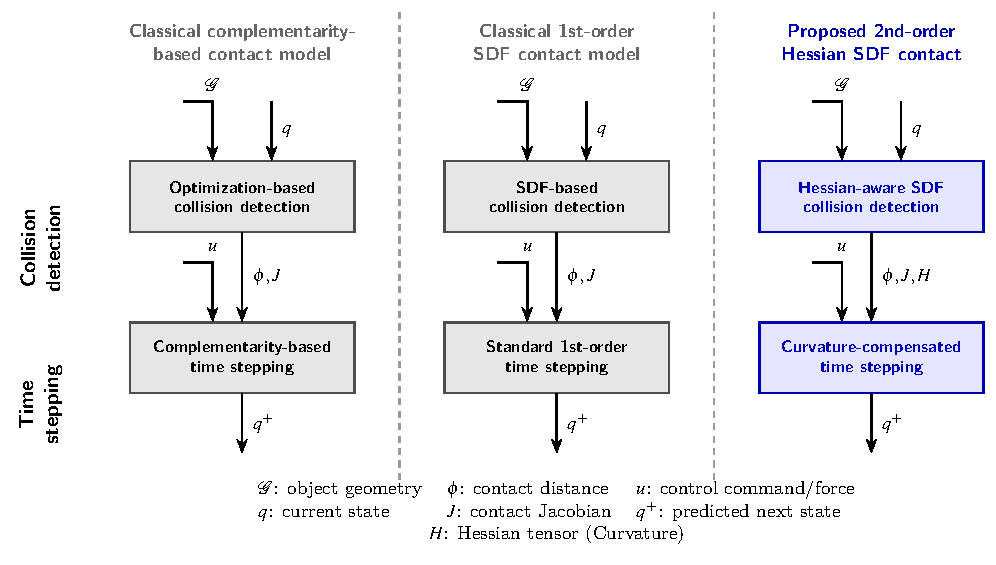
\includegraphics[width=\columnwidth]{flowchart_model.pdf}
    \caption{Three contact-modeling pipelines considered in this work: a classical mesh-based pipeline, a first-order SDF-based pipeline, and the proposed geometry-aware complementarity-based rigid-contact pipeline with curvature feedforward and regime-specific local representations}
    \label{fig:flowchart}
\end{figure}

Based on this modeling idea, the derivation proceeds through three closely connected steps. First, we analyze how the classical first-order local linearization leads to gap-prediction mismatch in high-curvature sliding and contact-state transitions. Second, we construct a local curvature representation from the SDF normal manifold and convert it into a geometric feedforward correction to the contact gap. Third, we introduce a contact-state-oriented configuration of local representations within a unified LCP chain, so that local geometric information enters the contact model in a regime-matched manner.

\subsection{Limitations of first-order local gap prediction in complementarity-based normal constraints}
In classical velocity-level complementarity-based contact treatment, in order to maintain non-penetration after a time step $\Delta t$, the velocity at the next step $\mathbf{v}^{l+1}$ is usually required to satisfy a first-order linearization of the local Signorini condition:
\begin{equation}
    \Phi(\mathbf{q}^{l+1}) \approx \Phi(\mathbf{q}^l) + \Delta t \, \mathbf{n}^T \mathbf{v}^{l+1} \geq 0.
\end{equation}
Here $\Phi(\mathbf{q}^l)$ is the current contact gap and $\mathbf{n}$ is the contact normal. For SDF-based point-contact models, the normal is obtained from the distance-field gradient. To remain consistent with the subsequent second-order curvature construction, we use the normalized unit normal
\begin{equation}
    \mathbf{n} = \frac{\nabla \Phi}{\|\nabla \Phi\|}.
\end{equation}

In the classical first-order model, when the time step is relatively large or the contact point undergoes rapid tangential sliding along a highly curved boundary, local tangent-plane extrapolation deviates from the true surface manifold. As a consequence, the right-hand-side gap prediction becomes systematically distorted. Such error can then be amplified by the nonsmooth complementarity equations into nonphysical impulses, which finally appear as high-frequency spikes and pulses in the velocity response.

\subsection{Local curvature characterization via the Weingarten map}
To capture the effect of local curvature on gap prediction, we elevate the local expansion of the contact gap from first to second order. Rather than differentiating the scalar distance field $\Phi$ directly to obtain a raw Hessian, we first construct the unit normal field
\begin{equation}
    \mathbf{n}(\mathbf{x}) = \frac{\nabla \Phi(\mathbf{x})}{\|\nabla \Phi(\mathbf{x})\|},
\end{equation}
and then apply central differencing to obtain the local curvature tensor
\begin{equation}
    \mathbf{W}(\mathbf{x}) \approx \nabla \mathbf{n}(\mathbf{x}).
\end{equation}
Accordingly, the second-order tensor used in this paper is essentially a discrete approximation of the Weingarten map on the SDF normal manifold, rather than a direct second derivative of the scalar field $\Phi$. For the local relative displacement $\mathbf{s} = \Delta t \, \mathbf{v}_{rel}$ over the current step, the second-order expansion of the contact gap becomes
\begin{equation}
    \Phi(\mathbf{q}^{l+1}) \approx \Phi(\mathbf{q}^{l}) + \mathbf{s}^T \mathbf{n} + \frac{1}{2}\mathbf{s}^T \mathbf{W}\mathbf{s}.
\end{equation}
Using a semi-implicit approximation of the current-step relative velocity then leads to the curvature compensation term
\begin{equation}
    C_{curve} = \frac{1}{2} (\Delta t)^2 \, \mathbf{v}_{rel}^T \mathbf{W} \mathbf{v}_{rel}.
\end{equation}

\subsection{Injection of local geometric feedforward into the normal LCP subproblem}
To make the injection location explicit, we first write the normal contact subproblem under time stepping in standard complementarity form. Suppose that there are $m$ active contact patches in the current step. Let all generalized velocities be stacked in $\mathbf{v}\in\mathbb{R}^{n_v}$, let the mass matrix be $\mathbf{M}$, and let the normal contact Jacobian be $\mathbf{J}_n\in\mathbb{R}^{m\times n_v}$, whose $i$th row satisfies
\begin{equation}
    (\mathbf{J}_n \mathbf{v})_i = \mathbf{n}_i^T \mathbf{v}_{rel,i},
\end{equation}
that is, it gives the relative normal velocity of the $i$th contact under the current generalized velocity. Temporarily retaining only the part associated with normal non-penetration, the Moreau--Jean-type discrete momentum update can be written as
\begin{equation}
    \mathbf{M}(\mathbf{v}^{l+1} - \mathbf{v}^{l}) = \Delta t\,\mathbf{f}^{l}_{ext} + \mathbf{J}_n^T \boldsymbol{\lambda}_n,
\end{equation}
where $\boldsymbol{\lambda}_n\in\mathbb{R}^{m}$ denotes the normal impulses of the active contacts over the time step. If the part without newly added normal impulses is denoted by the free velocity
\begin{equation}
    \mathbf{v}^{free} = \mathbf{v}^{l} + \mathbf{M}^{-1}\Delta t\,\mathbf{f}^{l}_{ext},
\end{equation}
then
\begin{equation}
    \mathbf{v}^{l+1} = \mathbf{v}^{free} + \mathbf{M}^{-1}\mathbf{J}_n^T \boldsymbol{\lambda}_n.
\end{equation}

Applying the first-order linearized Signorini non-penetration condition to all active contacts yields
\begin{equation}
    \mathbf{w}_n = \boldsymbol{\Phi} + \Delta t\,\mathbf{J}_n \mathbf{v}^{l+1} \ge 0,
\end{equation}
where $\boldsymbol{\Phi}=[\Phi_1,\ldots,\Phi_m]^T$ collects the normal gaps of all patches at the current time. Together with the complementarity conditions
\begin{equation}
    \boldsymbol{\lambda}_n \ge 0,\qquad
    \mathbf{w}_n \ge 0,\qquad
    \boldsymbol{\lambda}_n^T\mathbf{w}_n = 0,
\end{equation}
we obtain the standard normal LCP subproblem
\begin{equation}
    \mathbf{w}_n
    =
    \underbrace{\Delta t\,\mathbf{J}_n\mathbf{M}^{-1}\mathbf{J}_n^T}_{\mathbf{A}_n}
    \boldsymbol{\lambda}_n
    +
    \underbrace{\left(\boldsymbol{\Phi} + \Delta t\,\mathbf{J}_n \mathbf{v}^{free}\right)}_{\mathbf{b}_n},
    \qquad
    0 \le \boldsymbol{\lambda}_n \perp \mathbf{w}_n \ge 0.
\end{equation}
This normal LCP therefore solves for the normal impulse vector $\boldsymbol{\lambda}_n$ over a discrete time step so that the updated normal velocity and the predicted gap jointly satisfy the Signorini-type non-penetration complementarity condition. Here $\mathbf{A}_n$ reflects the effective dynamical mapping induced by the coupling of mass distribution and contact Jacobian, while $\mathbf{b}_n$ collects the current geometric gaps and the free-motion prediction terms.

In the full frictional-contact system, tangential unknowns, friction cones, or bilateral constraints are usually assembled together with the normal block into a more general MLCP or block-complementarity system. The key point for the present work, however, is that local geometric feedforward is injected only into the normal non-penetration channel and does not rewrite the left-hand dynamical coupling block itself. It is therefore sufficient to modify $\mathbf{b}_n$ without changing the structure, sparsity, or solution process of $\mathbf{A}_n$.

This choice is not merely an engineering convenience; it is dictated by the discrete model itself. If the second-order curvature term were treated as an endogenous part of the unknown velocity, a more rigorous expression would be
\begin{equation}
    C_{curve,i}(\mathbf{v}^{l+1})
    =
    \frac{1}{2}(\Delta t)^2
    (\mathbf{v}_{rel,i}^{l+1})^T
    \mathbf{W}_i
    \mathbf{v}_{rel,i}^{l+1},
\end{equation}
where $\mathbf{v}_{rel,i}^{l+1}$ itself depends on the unknown generalized velocity $\mathbf{v}^{l+1}$. Once substituted into
\begin{equation}
    \mathbf{v}^{l+1}
    =
    \mathbf{v}^{free}
    +
    \mathbf{M}^{-1}\mathbf{J}_n^T \boldsymbol{\lambda}_n,
\end{equation}
the complementarity residual becomes
\begin{equation}
    \mathbf{w}_n
    =
    \boldsymbol{\Phi}
    +
    \mathbf{c}_{curve}(\boldsymbol{\lambda}_n)
    +
    \Delta t\,\mathbf{J}_n\mathbf{v}^{free}
    +
    \Delta t\,\mathbf{J}_n\mathbf{M}^{-1}\mathbf{J}_n^T\boldsymbol{\lambda}_n,
\end{equation}
where $\mathbf{c}_{curve}(\boldsymbol{\lambda}_n)$ is already quadratic in the unknown impulse. In other words, once curvature correction is truly coupled into the left-hand unknowns, the original linear normal complementarity subproblem becomes a nonlinear complementarity problem (NCP), which no longer belongs to the standard LCP class targeted by the current solution chain. The objective of this paper is not to design a new nonlinear contact solver, but to introduce a minimally invasive geometric correction on top of the existing LCP chain; therefore, the curvature term must be frozen as an explicit feedforward quantity known at the current step.

Directly modifying the dynamical matrix on the left-hand side would also undermine the stability and reusability of the underlying LCP structure. To preserve the complementarity equations, we adopt a parasitic right-hand-side injection strategy and write second-order geometric information into the effective contact gap as a feedforward bias:
\begin{equation}
    \Phi_{eff} = \Phi + C_{curve}.
\end{equation}

Stacking all patch-wise curvature corrections into $\mathbf{c}_{curve}=[C_{curve,1},\ldots,C_{curve,m}]^T$ gives
\begin{equation}
    \boldsymbol{\Phi}_{eff} = \boldsymbol{\Phi} + \mathbf{c}_{curve},
\end{equation}
so that the original first-order non-penetration condition can be rewritten as
\begin{equation}
    \mathbf{w}_n^{eff} = \boldsymbol{\Phi}_{eff} + \Delta t\,\mathbf{J}_n \mathbf{v}^{l+1} \ge 0.
\end{equation}
Substituting back into the velocity-eliminated form yields the injected normal LCP
\begin{equation}
    \mathbf{w}_n^{eff}
    =
    \mathbf{A}_n \boldsymbol{\lambda}_n
    +
    \underbrace{\left(\boldsymbol{\Phi}_{eff} + \Delta t\,\mathbf{J}_n \mathbf{v}^{free}\right)}_{\mathbf{b}_n^{eff}}
    =
    \mathbf{A}_n \boldsymbol{\lambda}_n + \mathbf{b}_n + \mathbf{c}_{curve},
    \qquad
    0 \le \boldsymbol{\lambda}_n \perp \mathbf{w}_n^{eff} \ge 0.
\end{equation}

Accordingly, the term ``injection'' in this paper means the following in mathematical terms: \textbf{the left-hand LCP matrix $\mathbf{A}_n$ is kept unchanged, and the curvature-based local prediction $\mathbf{c}_{curve}$ is added only to the right-hand term $\mathbf{b}_n$.} This has three immediate benefits. First, the matrix assembly, preconditioning structure, and complementarity iteration procedure of the underlying solver remain unchanged. Second, when $\mathbf{c}_{curve}=\mathbf{0}$, the system automatically degenerates to the original first-order model. Third, curvature information is confined to patch-level gap prediction and influences only the decision of whether and when normal impulse is required, without introducing additional dynamical degrees of freedom.

From the perspective of numerical stability, this point is equally crucial. The matrix $\mathbf{A}_n=\Delta t\,\mathbf{J}_n\mathbf{M}^{-1}\mathbf{J}_n^T$ describes the global coupling among active contacts through effective mass transfer; its condition number, sparsity pattern, and block structure directly affect the convergence behavior of complementarity iterations. By contrast, the Hessian/Weingarten tensor comes from local differencing of a discrete SDF and is more sensitive to voxel resolution, interpolation error, nearest-point branch switching, and the geometric representative of each patch. If such second-order information were absorbed directly into the left-hand dynamical block, local geometric noise would propagate as a coupling perturbation over the entire contact system. Keeping it on the right-hand side, by contrast, amounts to correcting only the local gap prediction and contact-activation threshold of each patch. Its effect then remains patch-local and can be controlled conservatively through gating, clustering, and regime configuration. For this reason, the second-order curvature term is treated as a \textbf{geometric feedforward} rather than as a new dynamical coupling term.

That is, without rewriting the overall structure of the underlying complementarity module, the local second-order geometric prediction is injected into the main LCP equation through a correction of the right-hand-side contact gap. This preserves the backbone of the traditional nonsmooth contact framework while incorporating the kinematic look-ahead associated with highly curved surfaces into contact activation.

\subsection{Regime-oriented configuration of local geometric representations}
This paper does not assume that a single contact proxy is equally suitable for all contact scenarios. Instead, two types of local contact regimes are preconfigured for different contact types. The current implementation does not include a unified runtime contact classifier; the contact representation is explicitly specified at the case or application level. For smooth continuous-sliding contacts such as industrial cams, eccentric disk--roller followers, and the Onset Stress Benchmark, the implementation uses the \texttt{SlidingPatch} representation. In this regime, the contact set retains a persistent manifold identity over time, and representative queries, local fitting, and candidate filtering are used to maintain continuous patch-level geometric updates. For compact, impulse-dominated, or geometrically singular contacts such as Twin Gear and head-on impact, the implementation uses \texttt{CompactDiscrete}, where the goal of the patch is mainly duplicate removal, normal stabilization, and dominant-geometry preservation rather than temporal tracking of a continuous sliding manifold.

The core idea of this configuration strategy is that the curvature feedforward term does not guarantee positive gains for all contacts by itself. It becomes stable and useful only when embedded in a local manifold representation matched to the contact type. For smooth continuous contact, persistent tracking of the local manifold is a prerequisite for curvature feedforward to produce a net gain. For nonsmooth, impulse-dominated, or branch-switching-intensive contact, by contrast, a more conservative compact discrete representation is often more effective at suppressing nonphysical impulses induced by local geometric noise.

Figure \ref{fig:contact_regime_flow} further summarizes the two regime-specific processing paths currently supported by the implementation. The system first performs candidate-sample preprocessing, optionally with sample-side OBB/BVH broad-phase acceleration to reduce candidate-query cost. It then follows either the \texttt{SlidingPatch} or \texttt{CompactDiscrete} path according to the regime preset in the case or application. Finally, the corrected effective gaps are written back into the same LCP solution chain.

\begin{figure}[htbp]
    \centering
    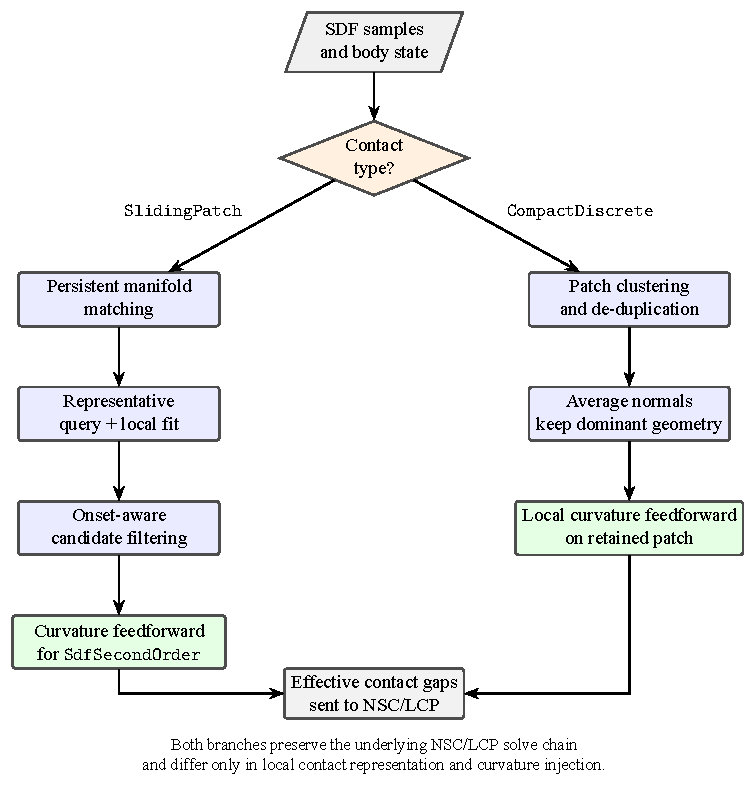
\includegraphics[width=\columnwidth]{flowchart_contact_regime.pdf}
    \caption{Regime-specific processing paths used in the current implementation. The pipeline is organized into candidate preprocessing, preconfigured manifold construction, and constraint injection. Candidate samples may first pass through an optional sample-side OBB/BVH broad-phase; depending on the regime preset in a given case or application, the solver then follows either the \texttt{SlidingPatch} path or the \texttt{CompactDiscrete} path, and both branches finally inject effective gaps into the same LCP solve chain}
    \label{fig:contact_regime_flow}
\end{figure}

\subsection{Patch-based reduction of the local contact manifold}
Because discrete sampling may generate multiple neighboring samples within the same local contact zone, directly feeding all SDF query results point-wise into the complementarity module can amplify normal noise and duplicate contacts into significant numerical jitter. To address this issue, we introduce a patch-level clustering strategy over the active contact set.

First, all candidate active samples are sorted by penetration depth. They are then clustered according to spatial proximity and normal consistency. For any candidate sample $\mathbf{x}_i$ and the representative sample $\mathbf{x}_k$ of an existing patch, the sample is merged into the same patch if
\begin{equation}
    \|\mathbf{x}_i - \mathbf{x}_k\| < r_{cluster},
\end{equation}
\begin{equation}
    \mathbf{n}_i \cdot \mathbf{n}_k > \cos \theta_{cluster},
\end{equation}
where $r_{cluster}$ is the spatial-radius threshold and $\theta_{cluster}$ is the normal-angle threshold.

Within each patch, the normal vector is averaged across samples and renormalized:
\begin{equation}
    \bar{\mathbf{n}}_k =
    \frac{\sum_{i \in M_k} \mathbf{n}_i}
         {\left\|\sum_{i \in M_k} \mathbf{n}_i\right\|}.
\end{equation}
The principal geometric quantities of the patch, however, are not fully averaged. For penetration depth $\Phi$, gradient, and curvature tensor $\mathbf{W}$, the values associated with the deepest sample in the patch are retained. Each patch is therefore ultimately represented by
\begin{equation}
    \left(\bar{\mathbf{n}}_k, \Phi_k^{deep}, \mathbf{W}_k^{deep}\right),
\end{equation}
which then enters the assembly of contact constraints in the complementarity module.

This treatment serves two purposes simultaneously. On the one hand, normal averaging reduces directional jitter caused by discrete point contact. On the other hand, retaining the deepest-sample values of $\Phi$ and Hessian avoids excessive smoothing of the dominant contact geometry and preserves the ability of curvature compensation to respond to the true geometrically dominant point of contact.

\subsection{Applicability conditions and failure boundaries}
The effectiveness of the present method relies on a clear set of local modeling assumptions: over a single time step, the active contact can be described by a local field with a single dominant normal, the SDF normal manifold is sufficiently smooth within the patch neighborhood, and the contact evolution does not involve violent nearest-point branch switching. In such scenarios, the main error of first-order gap prediction can be interpreted as a geometric mismatch caused by local tangent-plane extrapolation, and the Weingarten-based second-order feedforward can be introduced consistently into the right-hand side while remaining compatible with the original complementarity chain.

By contrast, when contact is dominated by $C^0$ edges, sharp corners, extremely small backlash, or competing nearest-point branches, the differential expansion of local point contact is no longer stable or consistent by itself. In that case, the curvature term should not be interpreted as a universally reliable correction. It can only act as auxiliary local information under the joint constraints of a conservative regime, patch reduction, and candidate filtering. This is precisely why \texttt{CompactDiscrete} is introduced and why regimes are configured at the case level. The present work does not solve runtime automatic regime identification, nor does it claim that one local representation is uniformly optimal across all contact scenarios.


\section{Computational Realization}
This section describes the computational realization of the local-geometry-aware contact model. The computational structure is organized around four aspects: discrete representation of local geometric fields on sparse narrow-band SDFs, coordinate transformation and packaging of patch-level geometric quantities, hierarchical acceleration for candidate-sample enumeration, and interface-level write-back of geometric feedforward into the complementarity solution chain. Overall, the realization follows the same principle as the methodology section: local geometric information only modifies the contact-constraint input and does not alter the dynamical structure of the underlying LCP module.

\subsection{Discrete representation of local geometric fields on sparse narrow-band SDFs}
The implementation uses the trilinear interpolation query interface provided by NanoVDB \cite{museth2021nanovdb} and employs a sparse narrow-band SDF (SNB-SDF) built around the geometric boundary as the underlying implicit representation. As shown in Fig. \ref{fig:snb_sdf}, only active voxels within the narrow band $|d|\le\tau$ are retained, while voxels far from the interface are pruned. This avoids the $\mathcal{O}(N^3)$ storage cost of dense voxel grids and focuses the queries of $\Phi$, $\nabla\Phi$, and local second-order geometric quantities on the neighborhoods that actually matter for contact.

\begin{figure}[htbp]
    \centering
    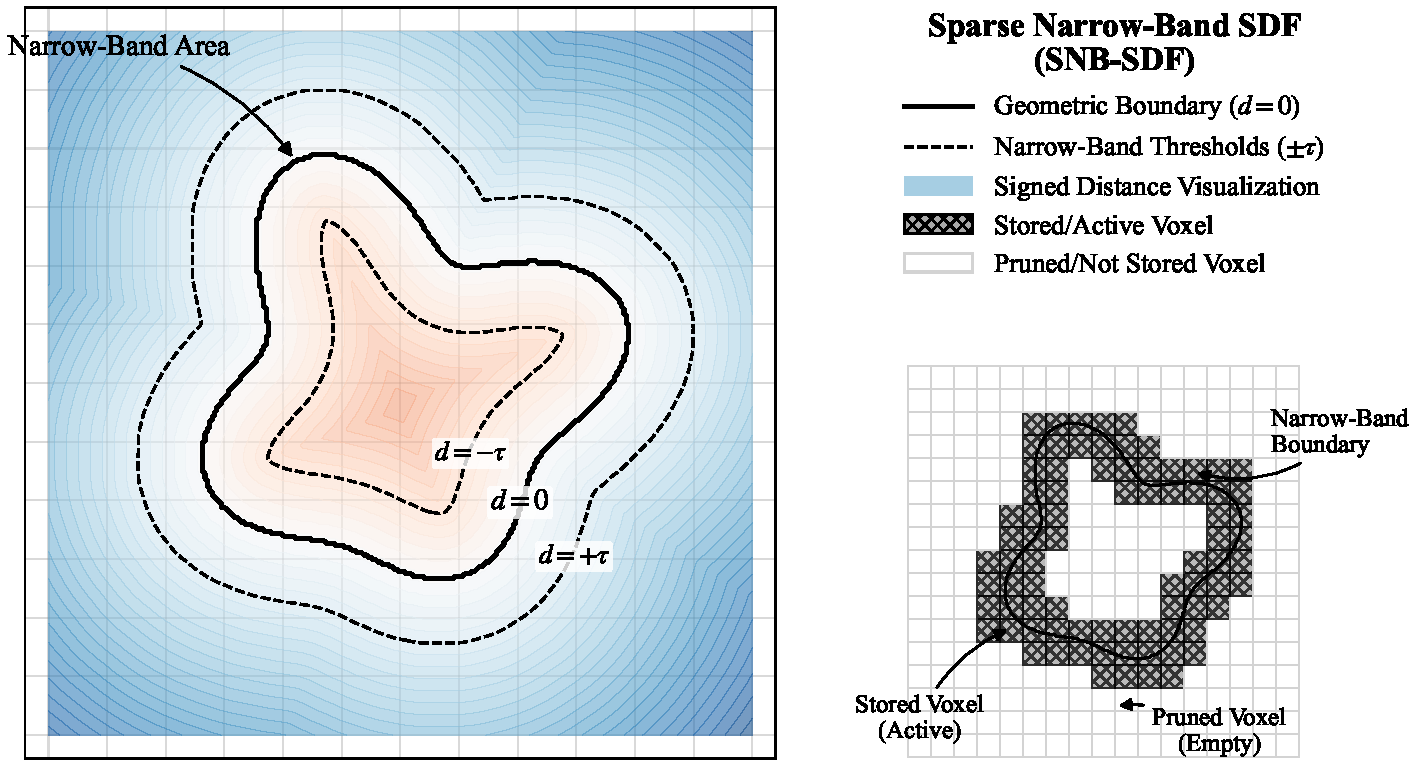
\includegraphics[width=0.98\linewidth]{SNB_SDF_Diagram_Compact_V2.pdf}
    \caption{Sparse narrow-band SDF (SNB-SDF). The left panel illustrates the continuous signed distance field, the geometric boundary $d=0$, and the narrow-band threshold $\pm\tau$; the lower-right panel illustrates the discrete voxel storage scheme, in which only voxels inside the narrow band are retained as active voxels while voxels far from the boundary are pruned}
    \label{fig:snb_sdf}
\end{figure}

Because discrete distance fields exhibit high-order discontinuities near voxel boundaries, the implementation does not compute the Hessian of the scalar distance field $\Phi$ directly. Instead, it first queries the unit normal field
\begin{equation}
    \mathbf{n} = \frac{\nabla \Phi}{\|\nabla \Phi\|},
\end{equation}
and then constructs the curvature tensor through central differencing:
\begin{equation}
    \mathbf{W} \approx \nabla \mathbf{n}.
\end{equation}
The differencing step size is chosen as
\begin{equation}
    h = 2 \cdot \text{voxel\_size}.
\end{equation}
The resulting $\mathbf{W}$ therefore corresponds to an approximation of the Weingarten map on the discrete SDF normal manifold.

\subsection{Coordinate mapping of local geometric quantities and patch encapsulation}
For each active contact sample, $\Phi$, the unit normal, and the curvature tensor $\mathbf{W}_M$ are first queried in model coordinates and then mapped into world coordinates through the rigid-body orientation matrix:
\begin{equation}
    \mathbf{W}_W = \mathbf{R}_{WM}\mathbf{W}_M\mathbf{R}_{WM}^T.
\end{equation}

During active-set construction, candidate samples are first filtered through a separating-velocity cutoff based on predicted normal relative velocity, so as to remove samples that are already clearly separating in the normal direction. The remaining candidates are then clustered into local patches according to spatial-radius and normal-angle thresholds. Patch normals are averaged and renormalized, whereas principal geometric quantities such as penetration depth $\Phi$, gradient, and Hessian are retained from the deepest sample. After this procedure, each patch is encapsulated as a local geometric proxy that can be inserted directly into contact-constraint assembly.

\subsection{Hierarchical candidate enumeration with OBB/BVH}
To reduce the query cost caused by dense surface sampling of follower bodies in continuous-sliding benchmarks, the implementation further introduces a static OBB/BVH broad phase on the sample side. This hierarchy is built in the follower's local coordinate frame. Each node stores a local OBB, a representative sample point, and the associated bounding radius. During simulation, it suffices to transform the representative point to world coordinates through the rigid-body pose and then into the model frame of the driving body's SDF for a lightweight $\Phi$ query.

Node-level pruning follows a conservative principle. A bounding-sphere lower bound of the driving geometry is first used to filter nodes that are clearly unable to contact. This is followed by conservative SDF pruning based on the representative point's $\Phi$ value, the node bounding radius, and a one-step motion margin. Only samples in unpruned leaf nodes proceed to accurate $(\Phi,\nabla\Phi)$ and, when needed, Hessian queries. The OBB/BVH layer therefore modifies only the candidate-enumeration strategy and does not alter leaf-level contact-sample construction, patch clustering, or the curvature-feedforward formula, which means that the final contact result is preserved.

This broad phase is enabled by default for the \texttt{SlidingPatch} path in continuous-sliding benchmarks such as the industrial cam, the eccentric disk--roller benchmark, and the Onset Stress Benchmark. For \texttt{CompactDiscrete} cases such as Twin Gear, where strong temporal coherence of local scanning is already present and contact switching is more compact, it is disabled by default and used only as an optional offline acceleration.

\subsection{Write-back of geometric feedforward into the right-hand side}
For each active patch, the implementation computes the second-order curvature compensation from the current-step relative contact-point velocity $\mathbf{v}_{rel}$:
\begin{equation}
    C_{curve} = \frac{1}{2} (\Delta t)^2 (\mathbf{v}_{rel})^T \mathbf{W}_{W} \mathbf{v}_{rel},
\end{equation}
and constructs the corrected effective contact gap
\begin{equation}
    \Phi_{eff} = \Phi + C_{curve}.
\end{equation}

The resulting $\Phi_{eff}$ is then written back into the contact-constraint interface and enters the underlying complementarity module as part of the right-hand side of the LCP equations. In this way, the computational realization preserves the parasitic right-hand-side injection structure introduced in the methodology: rather than altering the complementarity solution chain itself, it modifies the contact-constraint input through local geometric feedforward.

Algorithms \ref{alg:slidingpatch} and \ref{alg:compactdiscrete} summarize the computational paths of the two local contact representations. They share the same underlying LCP chain but differ fundamentally in candidate-sample screening, patch-level geometric encapsulation, and the conditions under which curvature terms are enabled.

\begin{algorithm}[htbp]
\caption{\texttt{SlidingPatch} pipeline for smooth continuous contact}
\label{alg:slidingpatch}
\begin{algorithmic}[1]
\Require Sample set $\mathcal{S}$, previous manifold $\mathcal{M}^{-}$, SDF interface
\Statex \textbf{Mode:} \texttt{SdfFirstOrder} or \texttt{SdfSecondOrder}
\Ensure Active contact patches with effective gaps $\Phi_{eff}$
\State Query $(\Phi,\nabla \Phi)$ for each sample in $\mathcal{S}$
\State Discard candidates failing the separating-velocity cutoff
\State Cluster the remaining candidates into local patches
\State Match current patches with $\mathcal{M}^{-}$ to preserve persistent-manifold identity
\State Update representative points through representative queries and local geometric fitting
\State Reject prematurely activated candidates that fail onset-aware filtering
\If{the current mode is \texttt{SdfSecondOrder}}
    \State Query the Hessian / Weingarten tensor at the representative geometry
    \State Compute $C_{curve} \gets \frac{1}{2}(\Delta t)^2 \mathbf{v}_{rel}^{T}\mathbf{W}\mathbf{v}_{rel}$
    \State Set $\Phi_{eff} \gets \Phi + C_{curve}$
\Else
    \State Set $\Phi_{eff} \gets \Phi$
\EndIf
\State Write the active patches into the LCP contact container
\end{algorithmic}
\end{algorithm}

\begin{algorithm}[htbp]
\caption{\texttt{CompactDiscrete} pipeline for compact or singular contact}
\label{alg:compactdiscrete}
\begin{algorithmic}[1]
\Require Sample set $\mathcal{S}$, SDF interface
\Statex \textbf{Mode:} \texttt{SdfFirstOrder} or \texttt{SdfSecondOrder}
\Ensure Compact active patch set retaining dominant geometry
\State Query $(\Phi,\nabla \Phi)$ for each sample in $\mathcal{S}$
\State Discard candidates failing the separating-velocity cutoff
\State Cluster the remaining candidates using spatial-radius and normal-angle thresholds
\State Average normals within each patch
\State Retain dominant/deepest geometry for $\Phi$, gradient, and Hessian
\State Truncate the active set according to the preset compact-patch budget
\If{the current mode is \texttt{SdfSecondOrder}}
    \State Compute local $C_{curve}$ on the retained patch geometry
    \State Set $\Phi_{eff} \gets \Phi + C_{curve}$
\Else
    \State Set $\Phi_{eff} \gets \Phi$
\EndIf
\State Write the compact active patches into the LCP contact container
\end{algorithmic}
\end{algorithm}


\section{Multibody Simulation Experiments}
To validate the local-geometry-aware complementarity-based rigid-contact modeling strategy developed above, the experiments in this section are organized along the progression of ``basic correctness, extended correctness, continuous-contact capability, industrial-scale performance, remaining limitations, and computational efficiency.'' The first two head-on collision cases are used to verify the correctness of pure impulse transfer. This is followed by the eccentric disk--roller and Onset Stress benchmarks, which assess long-term adherence and contact-onset behavior in smooth continuous contact. An industrial cam benchmark is then used to evaluate accuracy and stability for complex engineering geometry. The Twin Gear case is used to expose the remaining limitations, and a final runtime comparison summarizes the evidence that, under regime-matched configurations, computational efficiency and contact-response accuracy can coexist. It should be stressed that these experiments do not aim to prove that one single regime or one single local representation is universally optimal across all benchmarks. Instead, each case is run under a preset regime matched to its contact state in order to assess the effectiveness and limitations of the proposed modeling strategy across different scenarios.

Unless otherwise stated, all compared methods are run in the same rigid-body dynamics environment and share the same time-stepping framework, external loading, output sampling, and benchmark-specific time-step settings. \texttt{Native Mesh} denotes the original mesh-based contact representation. \texttt{SdfFirstOrder} and \texttt{SdfSecondOrder} share the same SDF-based contact pipeline and differ only in the level of local geometric information used: the former uses only distance and first-order normal information, whereas the latter further introduces curvature feedforward. The direct difference between \texttt{SdfFirstOrder} and \texttt{SdfSecondOrder} therefore measures the incremental benefit of curvature feedforward, while the difference between mesh and the SDF path should be interpreted as an end-to-end comparison between the full local-geometry-aware modeling stack and the native contact representation. For continuous-sliding cases, the persistent manifold, local fitting, candidate filtering, and patch reduction together form the complete \texttt{SlidingPatch} path. The corresponding benchmarks therefore validate the effectiveness of the full modeling stack rather than the isolated effect of any single module.

Analytical references are used whenever available. When closed-form references are not available, external reference data independent of the present SDF pipeline are used instead. Specifically, the head-on collision and eccentric disk--roller cases use analytical references; the Onset Stress benchmark uses a piecewise analytical reference derived from the benchmark geometry and given kinematics; the industrial cam uses third-party reference curve data; and Twin Gear uses a commercial industrial software baseline. All runtimes are reported as end-to-end wall-clock time, so the broad phase, patch construction, and geometric-feedforward preprocessing in the SDF path are all included in the total runtime.

To ensure objective evaluation of computational cost and performance, all simulations were executed on the same high-performance workstation. The main hardware configuration consisted of an \textbf{AMD Ryzen 9 5900X 12-Core processor} and \textbf{16 GB of memory}. The software environment ran on Linux under Windows Subsystem for Linux 2 (WSL2). The code was compiled natively using GCC together with CMake, with a consistent highest-level optimization option such as \texttt{-O3} enabled globally.

\subsection{Basic correctness: head-on equal-sphere impact}
We first construct the most basic pure-impulse verification case: two spheres with identical radius and mass collide head-on along the same line. No gravity is applied, the friction coefficient is set to zero, and a translational joint constrains both bodies to a single translation direction so that lateral drift and attitude perturbations are excluded. The initial condition is set such that sphere A moves toward initially stationary sphere B with unit speed. Under perfectly elastic impact, the theoretical outcome is the classical one-dimensional velocity exchange: sphere A stops after impact and sphere B fully inherits the initial velocity of sphere A. Because the geometry, mass, and constraints are all analytically characterized, this case is appropriate as a basic physical-consistency test of the current shared SDF contact path in a pure-impulse setting rather than as an engineering-efficiency benchmark.

\begin{figure}[!t]
    \centering
    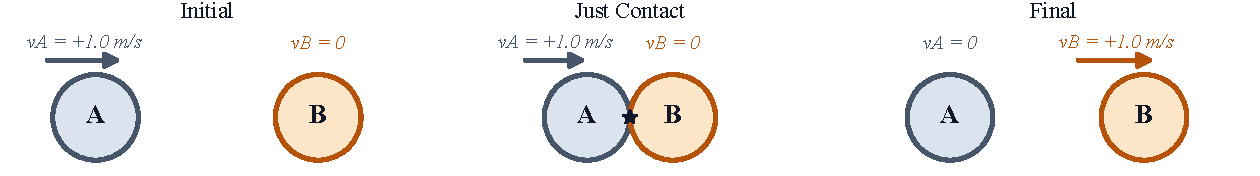
\includegraphics[width=\linewidth]{headon_equal_spheres_states.pdf}
    \caption{Three-stage model illustration of the equal-mass head-on collision case. From left to right: initial state, first contact, and final post-impact state. Velocity arrows indicate the direction and magnitude of the sphere velocities at each stage}
    \label{fig:headon_spheres_states}
\end{figure}

Figure \ref{fig:headon_spheres} shows the velocity histories of spheres A and B. On the current shared SDF contact path, both first-order and second-order SDF recover the ideal velocity exchange exactly in the discrete output: near the impact time, the velocity of sphere A jumps from $1.0$ m/s to $0.0$ m/s, while sphere B jumps from $0.0$ m/s to $1.0$ m/s. Their velocity RMSE relative to the analytical piecewise reference is therefore zero at the sampled output points.

By contrast, the native sphere contact still produces the correct final velocity exchange under the same time step, but exhibits a one-time-step switching delay in the discrete output, resulting in a velocity RMSE of $3.16\times10^{-2}$ m/s. This delay should be interpreted as a switching-time bias under the shared discrete step size rather than as an incorrect final impulse transfer. The result shows that the current SDF-based local-geometry-aware contact path can not only handle continuous sliding contact, but can also deliver correct momentum transfer in the most basic frictionless pure-impact setting, thereby establishing the physical-consistency foundation required for more general transient impact problems.

\begin{figure}[!t]
    \centering
    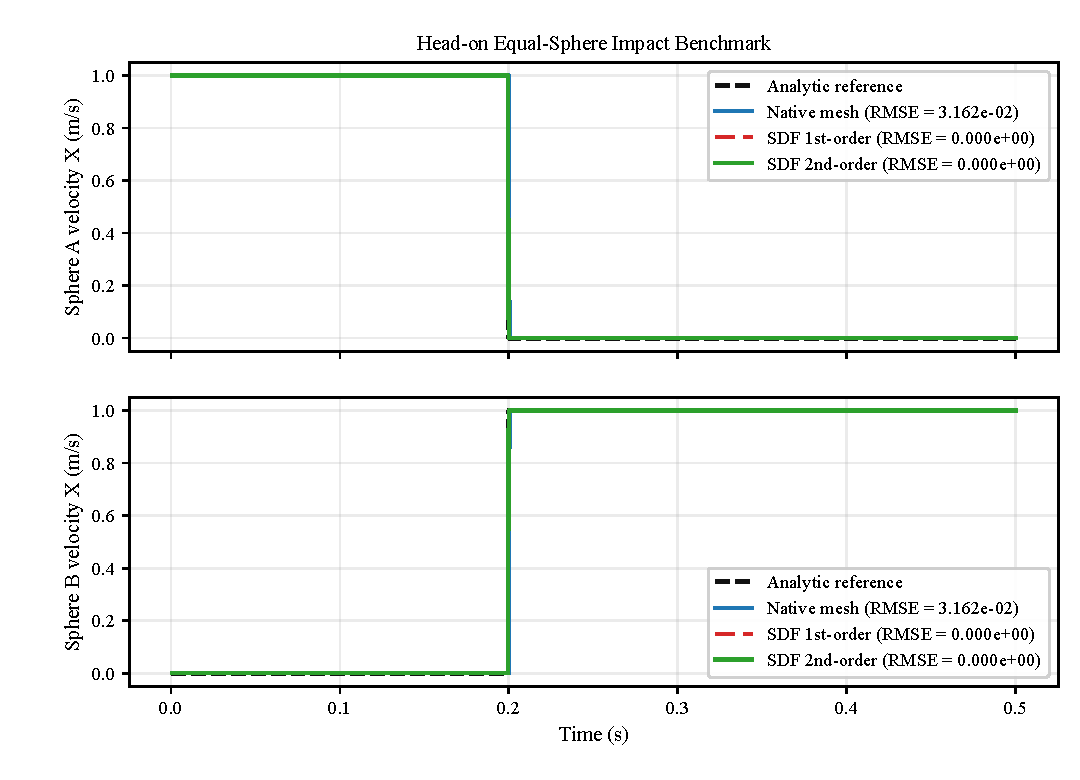
\includegraphics[width=0.94\linewidth]{headon_spheres_benchmark.pdf}
    \caption{Velocity histories for the equal-radius elastic head-on impact benchmark. Upper: sphere A. Lower: sphere B. The dashed black line denotes the analytical solution. Both SDF variants recover the ideal exchange, whereas the native mesh shows a switching lag of one time-step order}
    \label{fig:headon_spheres}
\end{figure}

\subsection{Extended correctness: head-on unequal-mass sphere impact}
To further confirm that the preceding conclusion is not limited to the special case of equal-mass velocity exchange, we construct an additional pure-impulse impact benchmark with equal radii but unequal masses. The two spheres keep the same radius, but sphere B is assigned twice the mass of sphere A. The initial condition is chosen such that sphere A is stationary and sphere B moves toward it along the constrained direction with velocity $-1.0$ m/s. Under perfectly elastic one-dimensional head-on impact, the analytical solution is
\[
v_A^+=-\frac{4}{3}\ \text{m/s},\qquad
v_B^+=-\frac{1}{3}\ \text{m/s}.
\]
This case shares the same zero-gravity, zero-friction, single-translation-joint setting as the equal-mass benchmark, but because the mass ratio is changed, the post-impact velocities are no longer a simple exchange. It is therefore a more appropriate test of whether the current shared SDF contact path truly obeys the analytical impulse law.

\begin{figure}[!t]
    \centering
    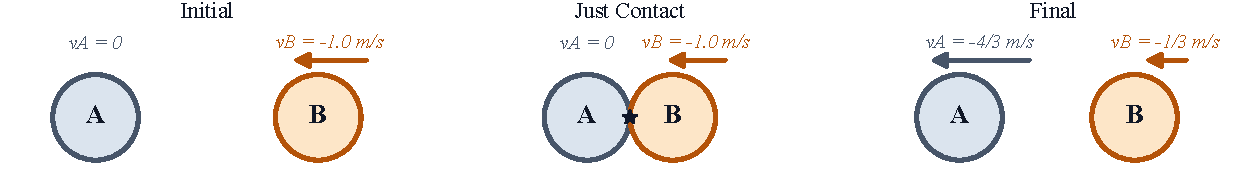
\includegraphics[width=\linewidth]{headon_unequal_mass_spheres_states.pdf}
    \caption{Three-stage model illustration of the unequal-mass head-on collision case. From left to right: initial state, first contact, and final state. Velocity arrows indicate the motion directions of spheres A and B together with the analytical post-impact velocities}
    \label{fig:headon_spheres_massratio_states}
\end{figure}

Figure \ref{fig:headon_spheres_massratio} shows the velocity histories of spheres A and B in the unequal-mass collision. The results indicate that the default shared SDF contact path also aligns pointwise with the analytical piecewise ground truth in this case: the post-impact velocities predicted by both first-order and second-order SDF converge to $-4/3$ m/s and $-1/3$ m/s, respectively, and the corresponding velocity RMSE values for the two spheres are about $2.6\times10^{-7}$. By contrast, the native sphere contact still produces the correct final post-impact velocity, but again exhibits a switching lag on the order of one discrete time step. The resulting velocity RMSE values are $4.22\times10^{-2}$ m/s for sphere A and $2.11\times10^{-2}$ m/s for sphere B. As in the equal-mass case, the discrepancy mainly reflects switching-time bias under the shared time-stepping configuration rather than an error in the final impulse law. This result demonstrates that the current shared SDF contact path reproduces not only equal-mass velocity exchange, but also the correct analytical impulse transfer for the more general unequal-mass head-on elastic impact.

\begin{figure}[!t]
    \centering
    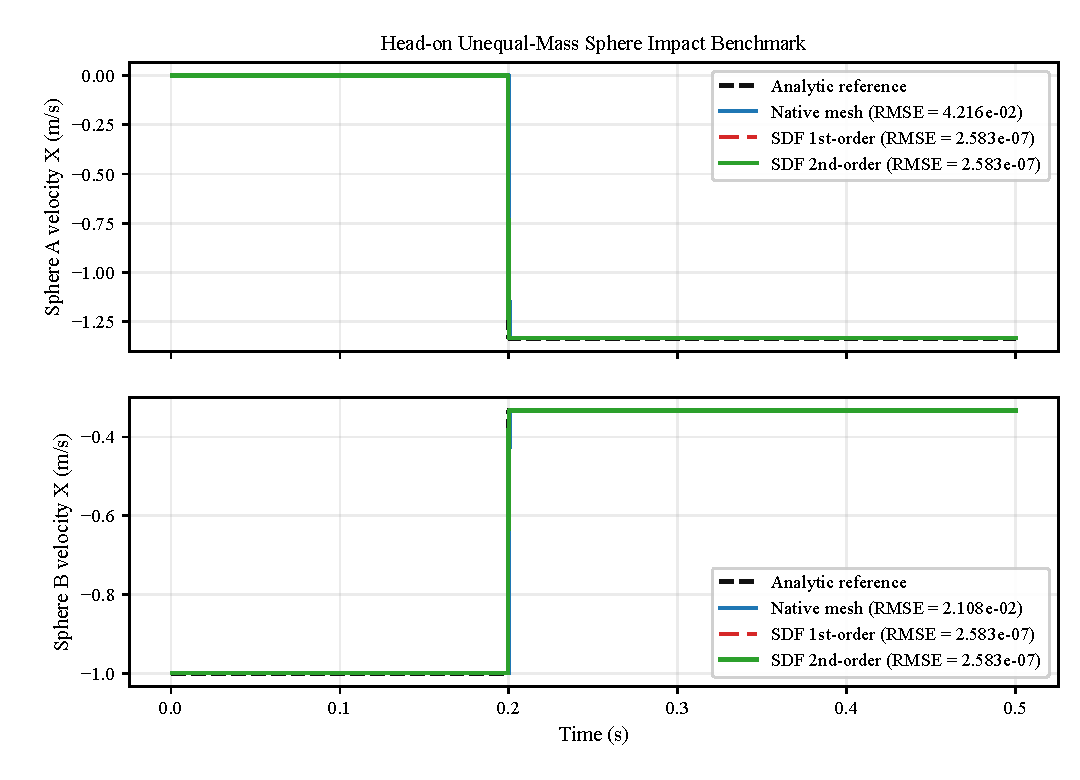
\includegraphics[width=0.94\linewidth]{headon_spheres_massratio_benchmark.pdf}
    \caption{Velocity histories for the unequal-mass elastic head-on impact benchmark, with sphere B twice as heavy as sphere A. Upper: sphere A. Lower: sphere B. The dashed black line denotes the analytical one-dimensional elastic-impact solution. Both SDF variants recover the correct post-impact velocities, while the native mesh again shows a switching lag of one time-step order}
    \label{fig:headon_spheres_massratio}
\end{figure}

\subsection{Continuous-contact capability: analytical roller benchmark (eccentric disk / roller follower)}
To separate the modeling capability for continuous sliding contact itself from possible CAD geometry error, local nonuniform sampling, and contact-switching effects in industrial cam systems, we further construct an analytically verifiable eccentric disk--roller follower benchmark. The driving body is a rigid disk with radius $R=30$ mm and eccentricity $e=6$ mm. The follower is a roller with radius $r=10$ mm constrained to translate along a vertical guide. The driving angular velocity is fixed at $\omega=-2$ rad/s, the simulation horizon is $T=\pi/2$ s, and the integration step size is $\Delta t=0.002$ s. For this geometry, the ideal no-separation motion satisfies
\[
y(t)=e\sin(\omega t)+\sqrt{(R+r)^2-(e\cos(\omega t))^2},
\]
so the numerical solution can be aligned pointwise with the analytical reference trajectory instead of relying on external commercial software output.

This benchmark shares the same LCP + SDF contact backbone as the other cases, but adopts an independent regime configuration better suited to smooth contact with a single dominant normal, with sample-side OBB/BVH broad phase enabled by default. The results are shown in Fig. \ref{fig:eccentric_roller}. Native mesh contact yields the smallest positional error, with position RMSE $3.0\times10^{-6}$ m and velocity RMSE $9.27\times10^{-4}$ m/s, but at a total runtime of $149.4$ s. First-order SDF reduces the runtime to $2.07$ s, with position RMSE $9.0\times10^{-6}$ m and velocity RMSE $6.94\times10^{-4}$ m/s. After introducing second-order curvature feedforward, second-order SDF further reduces the velocity RMSE to $6.88\times10^{-4}$ m/s while keeping nearly the same runtime ($2.23$ s), and limits the maximum velocity error to $1.20\times10^{-2}$ m/s, which is on the same order as the native mesh result.

The significance of this comparison is that it shows the complete \texttt{SlidingPatch} path itself can produce high-quality results with a substantial efficiency advantage in truly smooth and analytically solvable continuous sliding contact. Moreover, within the shared SDF path, second-order curvature feedforward provides a clear incremental accuracy gain over the first-order SDF formulation. In other words, in this regime-matched continuous-contact setting, higher response accuracy does not require a correspondingly large increase in computational cost. This result is complementary to the later Twin Gear benchmark: the present case shows that curvature feedforward is effective and efficient on smooth continuous manifolds, whereas Twin Gear reveals that a structural error floor remains near $C^0$ singular boundaries.

\begin{figure}[!t]
    \centering
    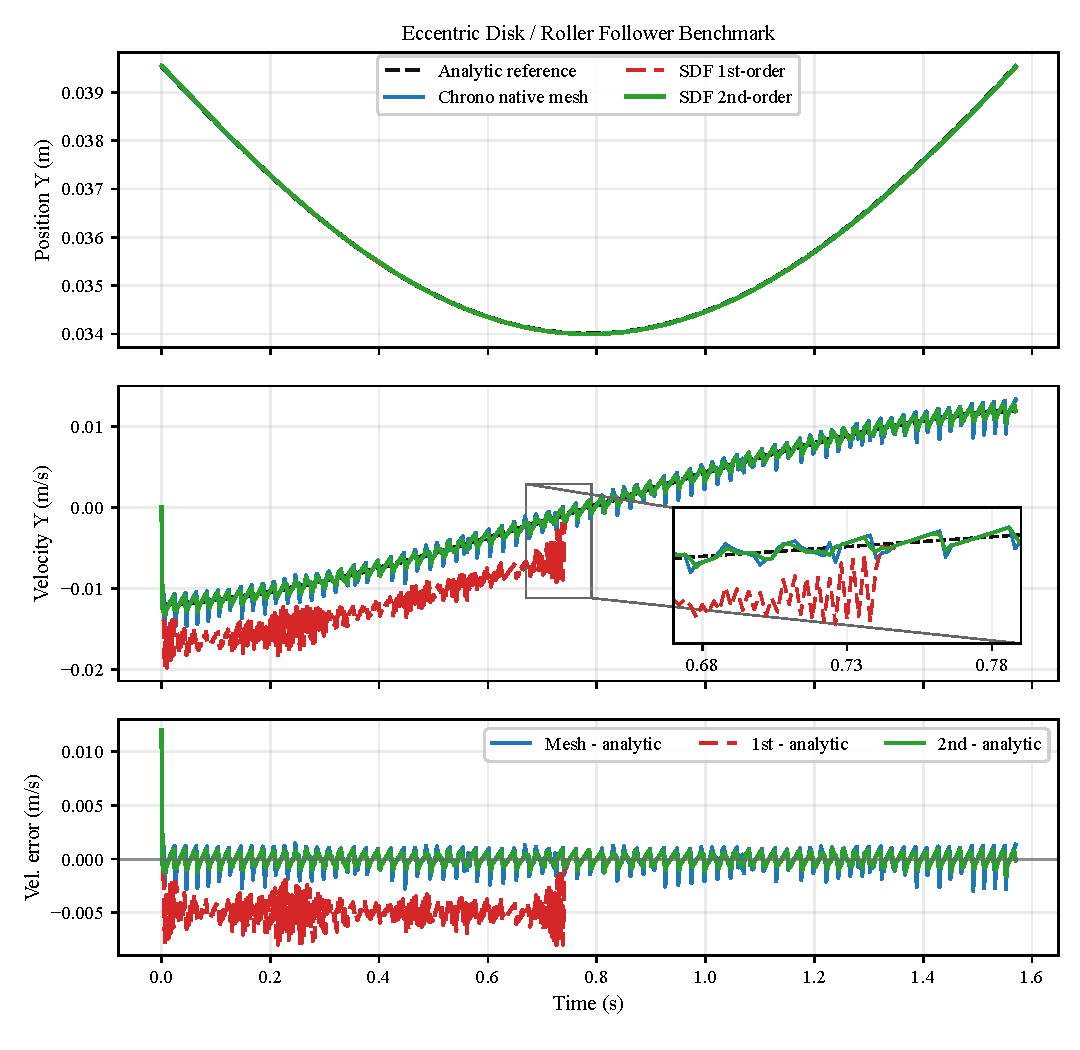
\includegraphics[width=0.94\linewidth]{eccentric_roller_benchmark.pdf}
    \caption{Analytical benchmark for an eccentric disk--roller follower. The upper, middle, and lower panels show displacement, velocity, and velocity error relative to the analytical reference, respectively. In this smooth continuous-sliding case, the second-order SDF reduces the velocity error while retaining runtime on the same order as the first-order SDF}
    \label{fig:eccentric_roller}
\end{figure}

\subsection{Contact-onset capability: Onset Stress benchmark (Onset Stress B)}
To further distinguish ``manifold-activation error at first contact'' from ``continuous-sliding error after contact has been established,'' we construct a Version B stress test by adding a weak follower return spring--damper to the positive-gap eccentric disk--roller model of Version A. The geometry remains smooth, the target onset time stays the same ($t_{\mathrm{on}}\approx 0.15$ s), and the same analytical reference is retained. The weak preload causes the follower to remain close to the envelope after contact onset instead of detaching in an approximately free-flight manner as in Version A. The model configuration is shown in Fig. \ref{fig:onset_model}.

\begin{figure}[!htbp]
    \centering
    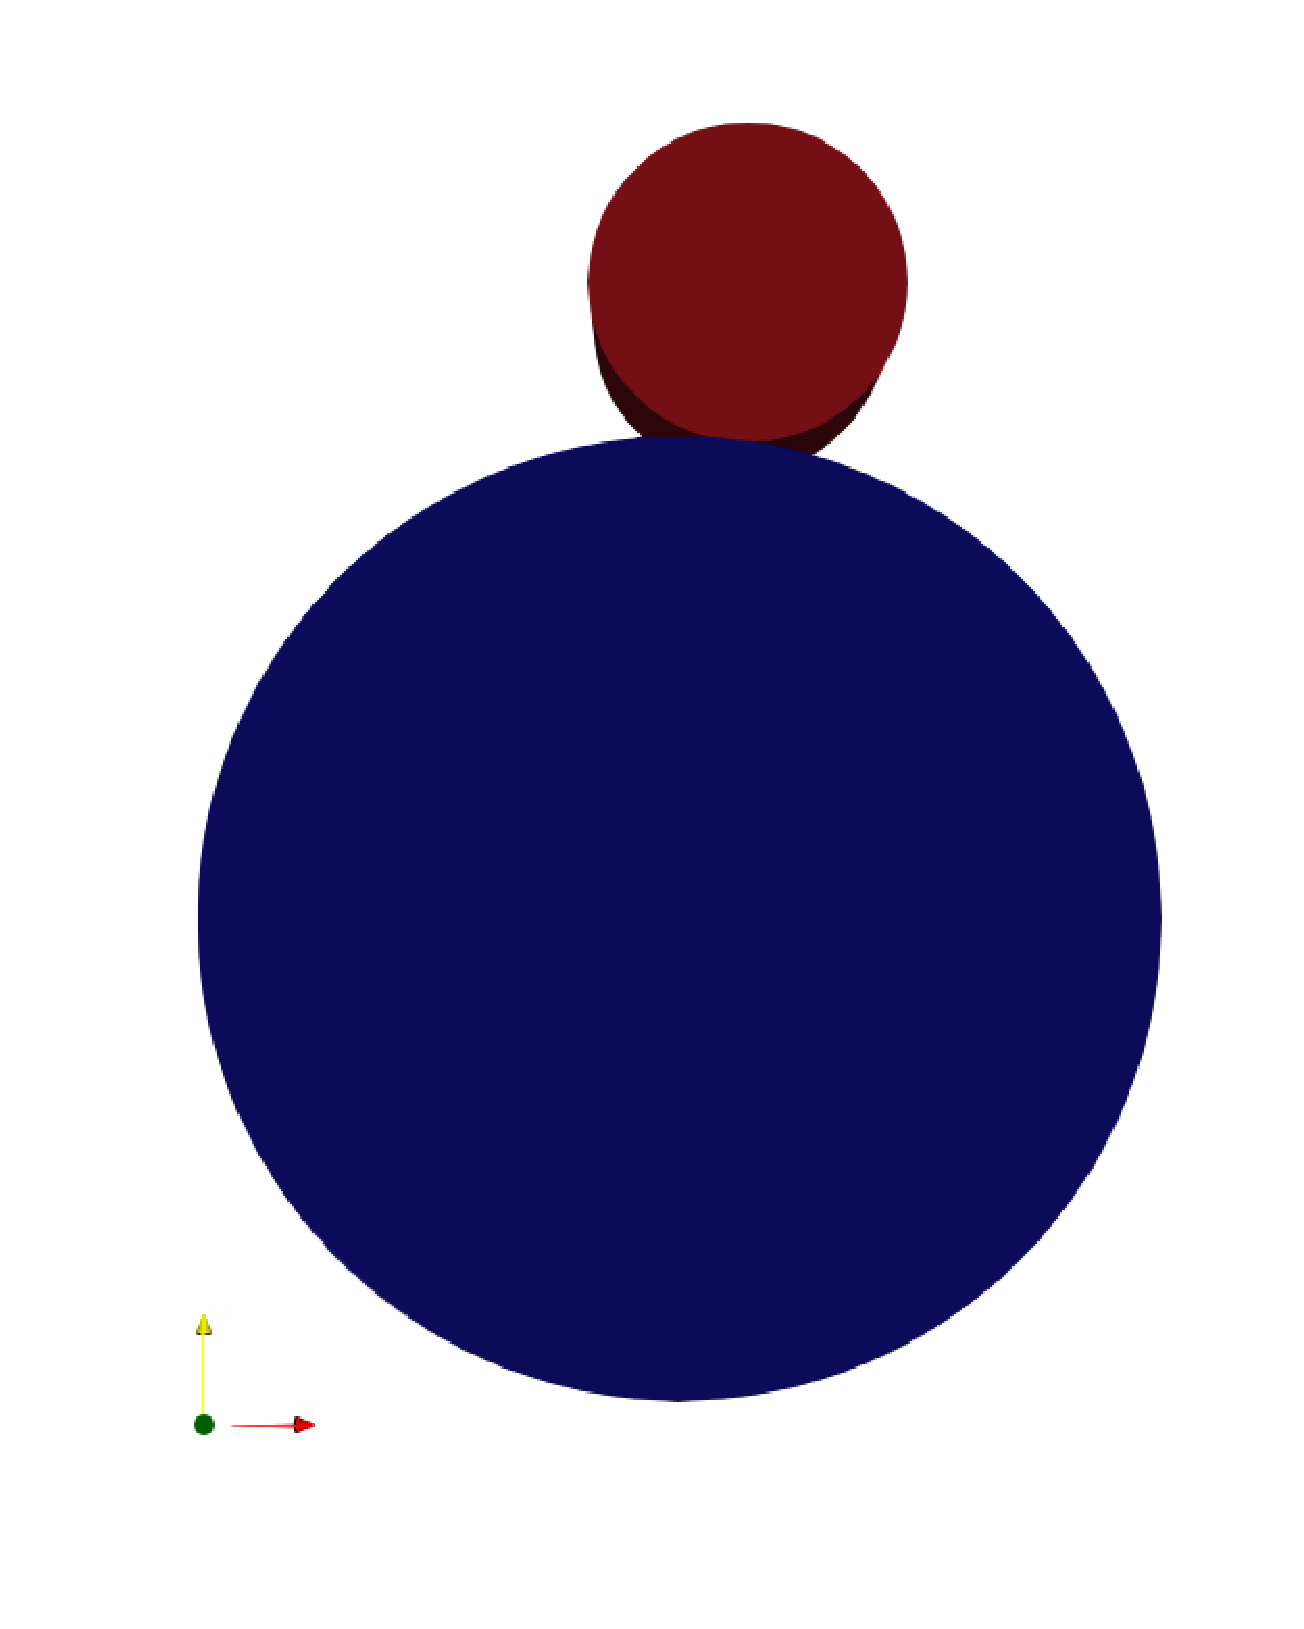
\includegraphics[width=0.54\linewidth]{onset.pdf}
    \caption{Model illustration of the Onset Stress B case. The figure shows the cam--roller system with a weakly preloaded return spring--damper, including the positive-gap initial state and the subsequent sustained-contact stage}
    \label{fig:onset_model}
\end{figure}

In the converged default setting, Version B uses $\Delta t = 0.001$ s, 32 dynamics substeps, an SDF voxel resolution of $100\,\mu$m, and follower return spring--damper parameters $k=670$ N/m and $c=47$ Ns/m, with sample-side OBB/BVH broad phase enabled by default. The results are shown in Fig. \ref{fig:onset_stress_b}. Native mesh contact yields a velocity RMSE of $8.59\times10^{-4}$ m/s and a total runtime of $111.5$ s. First-order SDF achieves a velocity RMSE of $8.43\times10^{-4}$ m/s with a total runtime of $35.4$ s, while second-order SDF further reduces the RMSE to $8.41\times10^{-4}$ m/s with a runtime of $36.4$ s. In other words, on this stress case designed specifically for sustained sliding after onset, both SDF curves already match and slightly exceed native mesh in terms of velocity RMSE after the introduction of continuous-contact-oriented candidate screening, local geometric fitting, and higher temporal resolution, with second-order SDF achieving the best result.

The significance of this result is that the persistent sliding manifold, local geometric fitting, and onset-aware candidate filtering added for continuous sliding do not merely ``appear effective'' in more complex industrial cam benchmarks, but genuinely recover long-term adherence in a controlled stress benchmark with analytically known onset time and an independently assessable sustained-contact phase. Combined with the runtime data, this also shows that the accuracy gain is not purchased by a dramatic increase in cost, but is achieved at a total runtime still far below that of native mesh contact. At the same time, the difference between first-order and second-order results indicates that curvature feedforward still provides an additional, though relatively moderate, incremental gain within this complete continuous-contact modeling stack. Compared with the eccentric benchmark, Version B places more emphasis on the difficulty of maintaining contact after transitioning from a free-gap state into contact; compared with the later Twin Gear benchmark, it avoids $C^0$ singular boundaries and nearest-point branch competition, and therefore provides a cleaner validation of local-geometry-aware modeling in continuous contact.

\begin{figure}[!t]
    \centering
    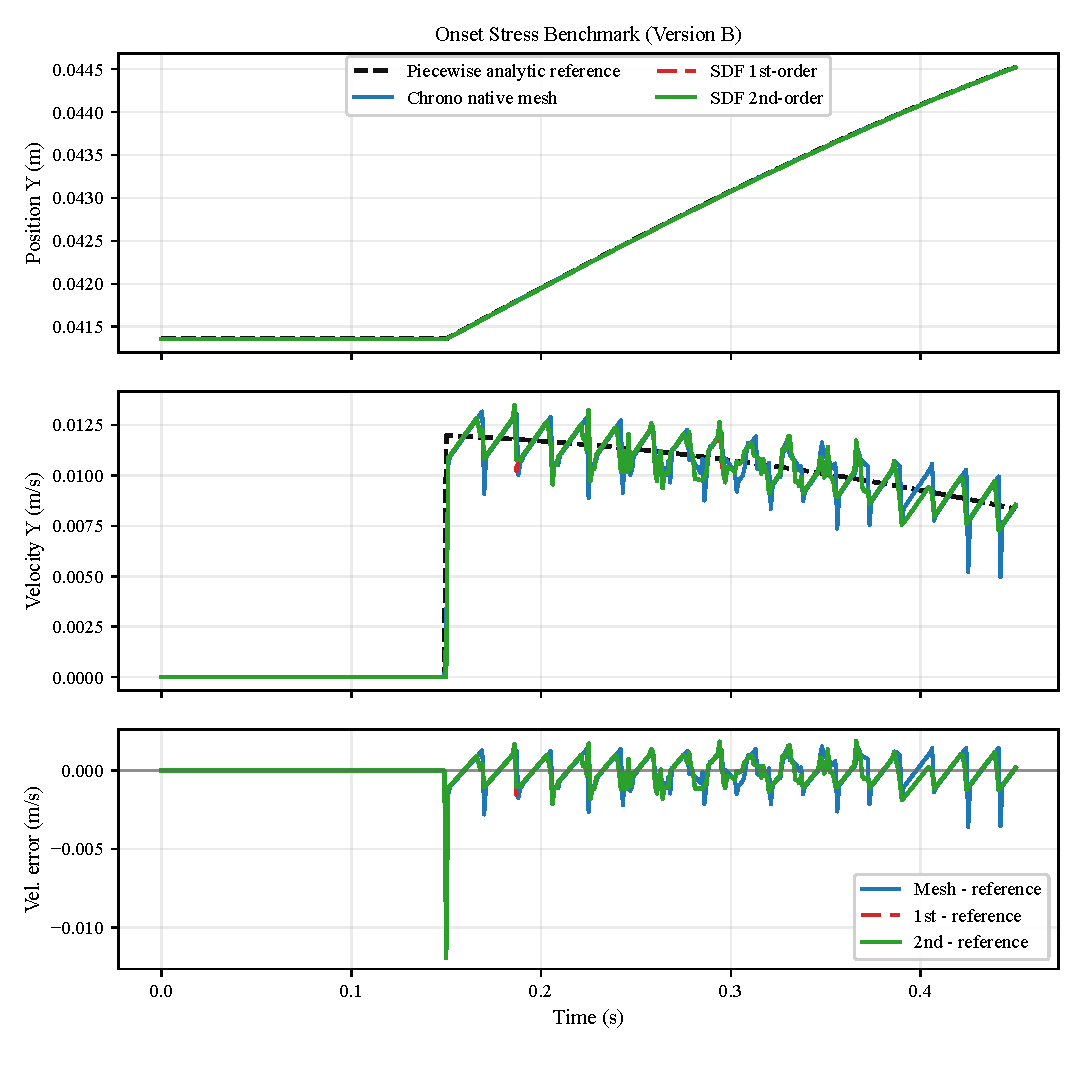
\includegraphics[width=0.94\linewidth]{onset_stress_benchmark.pdf}
    \caption{Onset Stress Benchmark Version B. The upper, middle, and lower panels show displacement, velocity, and velocity error relative to the piecewise analytical reference, respectively. In the sustained-sliding phase, both SDF variants match or slightly outperform native mesh in velocity RMSE, with the second-order SDF giving the best result}
    \label{fig:onset_stress_b}
\end{figure}

\clearpage

\subsection{Industrial-scale performance: cam under the base time step}
We now move to the continuous-contact response of an industrial cam--follower system under the base time step. Errors in this benchmark are measured against third-party reference curve data. The current setup uses the \texttt{SlidingPatch} contact representation, a base time step of $\Delta t = 0.005$ s, and an SDF voxel resolution of $4\times 10^{-4}$ m. This corresponds to a relatively fine temporal resolution, under which all three methods track the reference trajectory stably, making it appropriate for comparing error distributions and local peak suppression across different contact representations. The model states are shown in Fig. \ref{fig:cam_model}, where the three views from left to right correspond to the initial state, the instant of first contact, and the final simulation time.

\begin{figure}[!htbp]
    \centering
    \begin{minipage}[t]{0.32\linewidth}
        \centering
        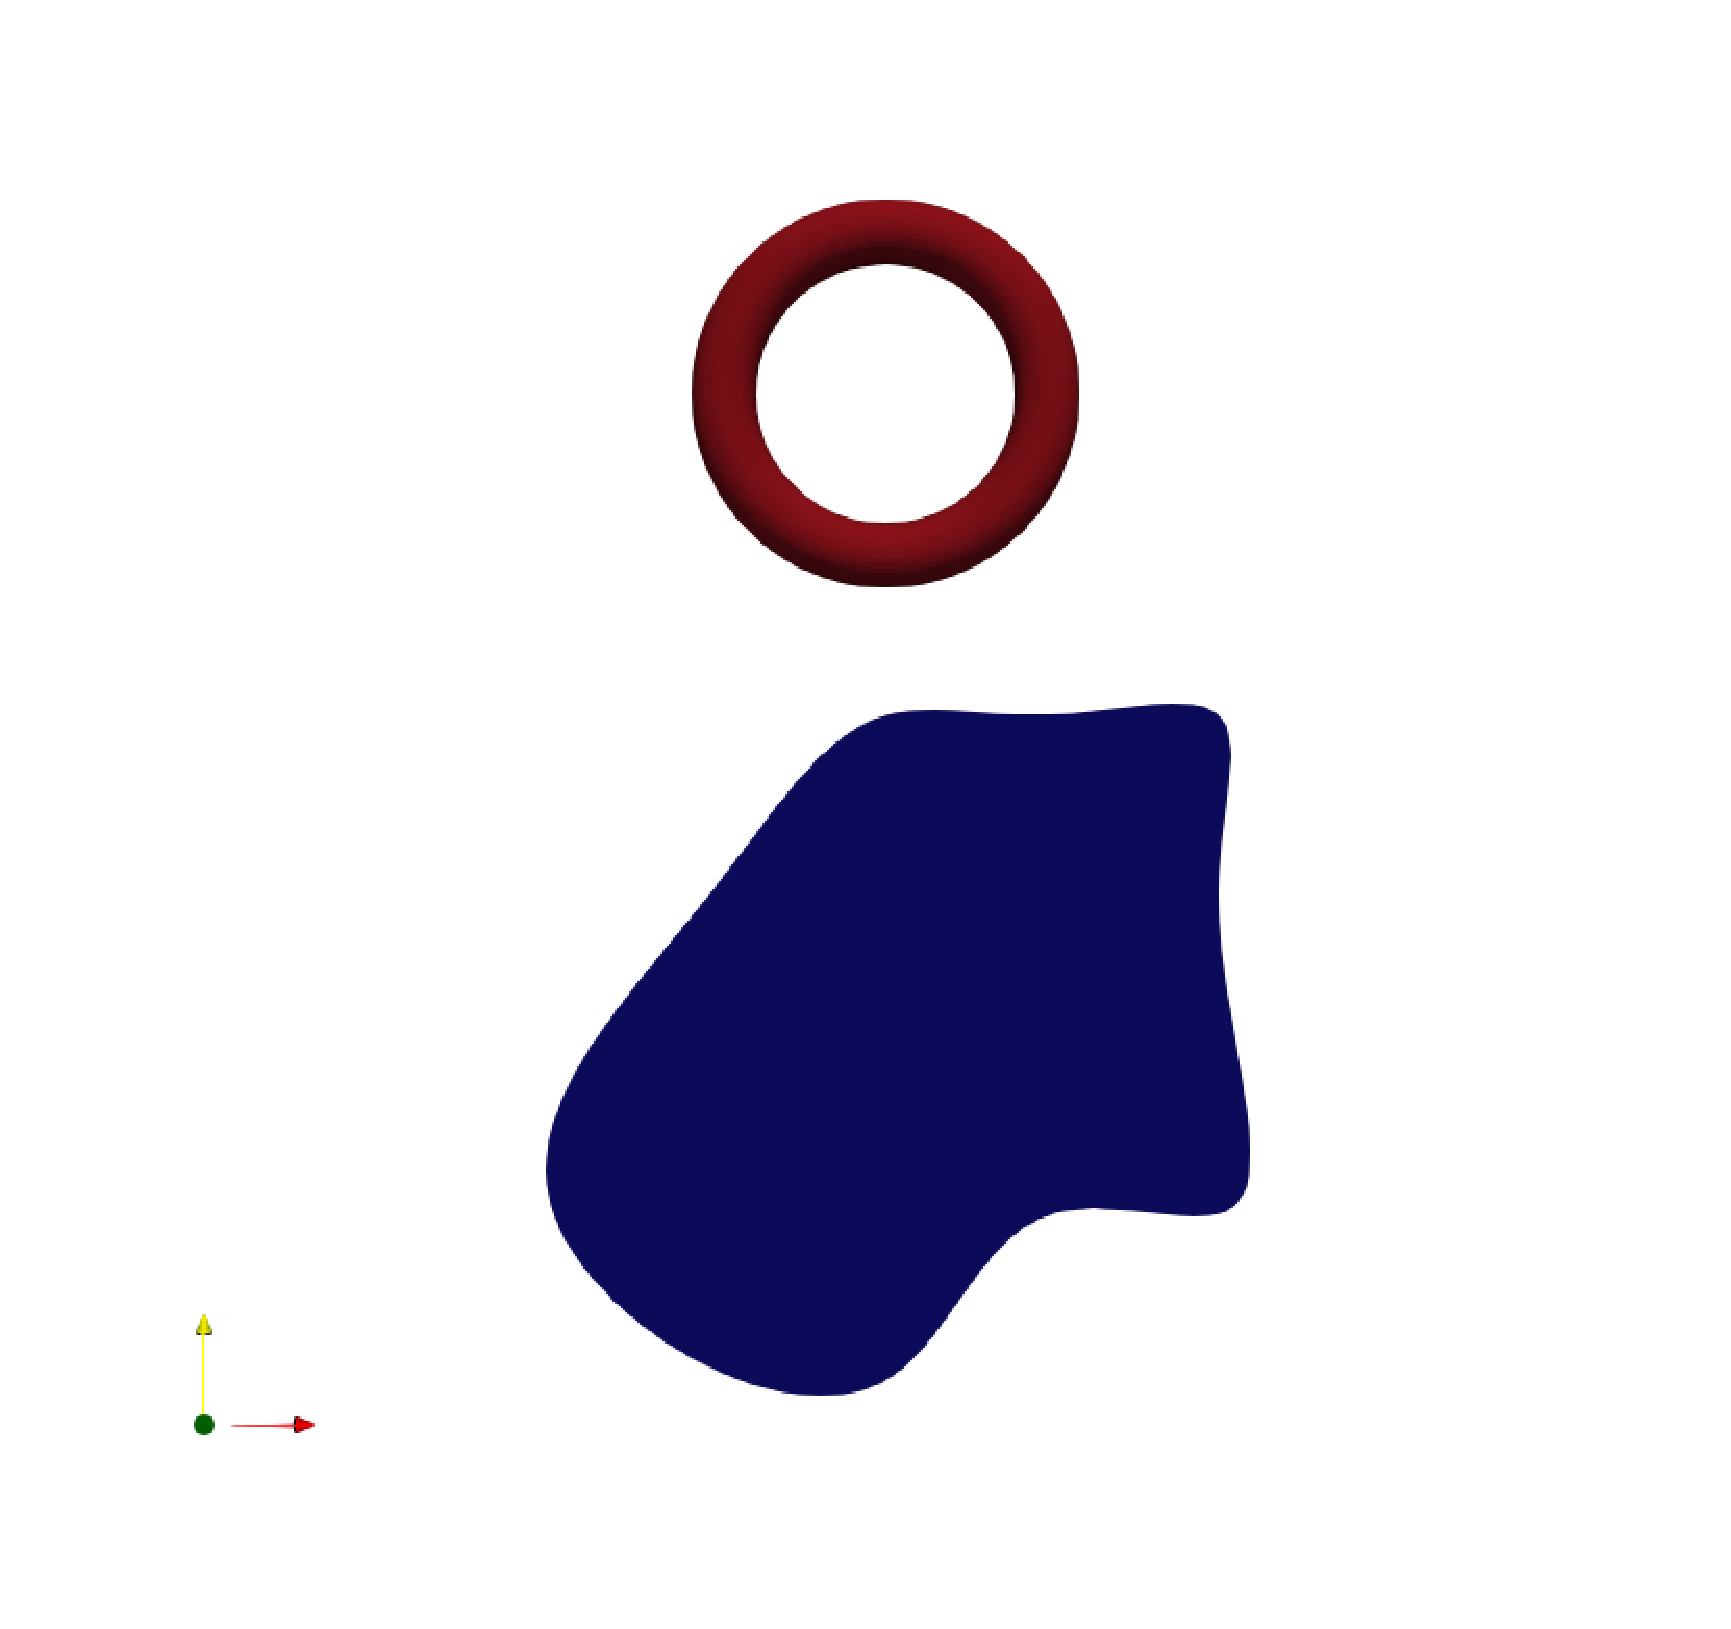
\includegraphics[width=\linewidth]{cam_0.pdf}
    \end{minipage}\hfill
    \begin{minipage}[t]{0.32\linewidth}
        \centering
        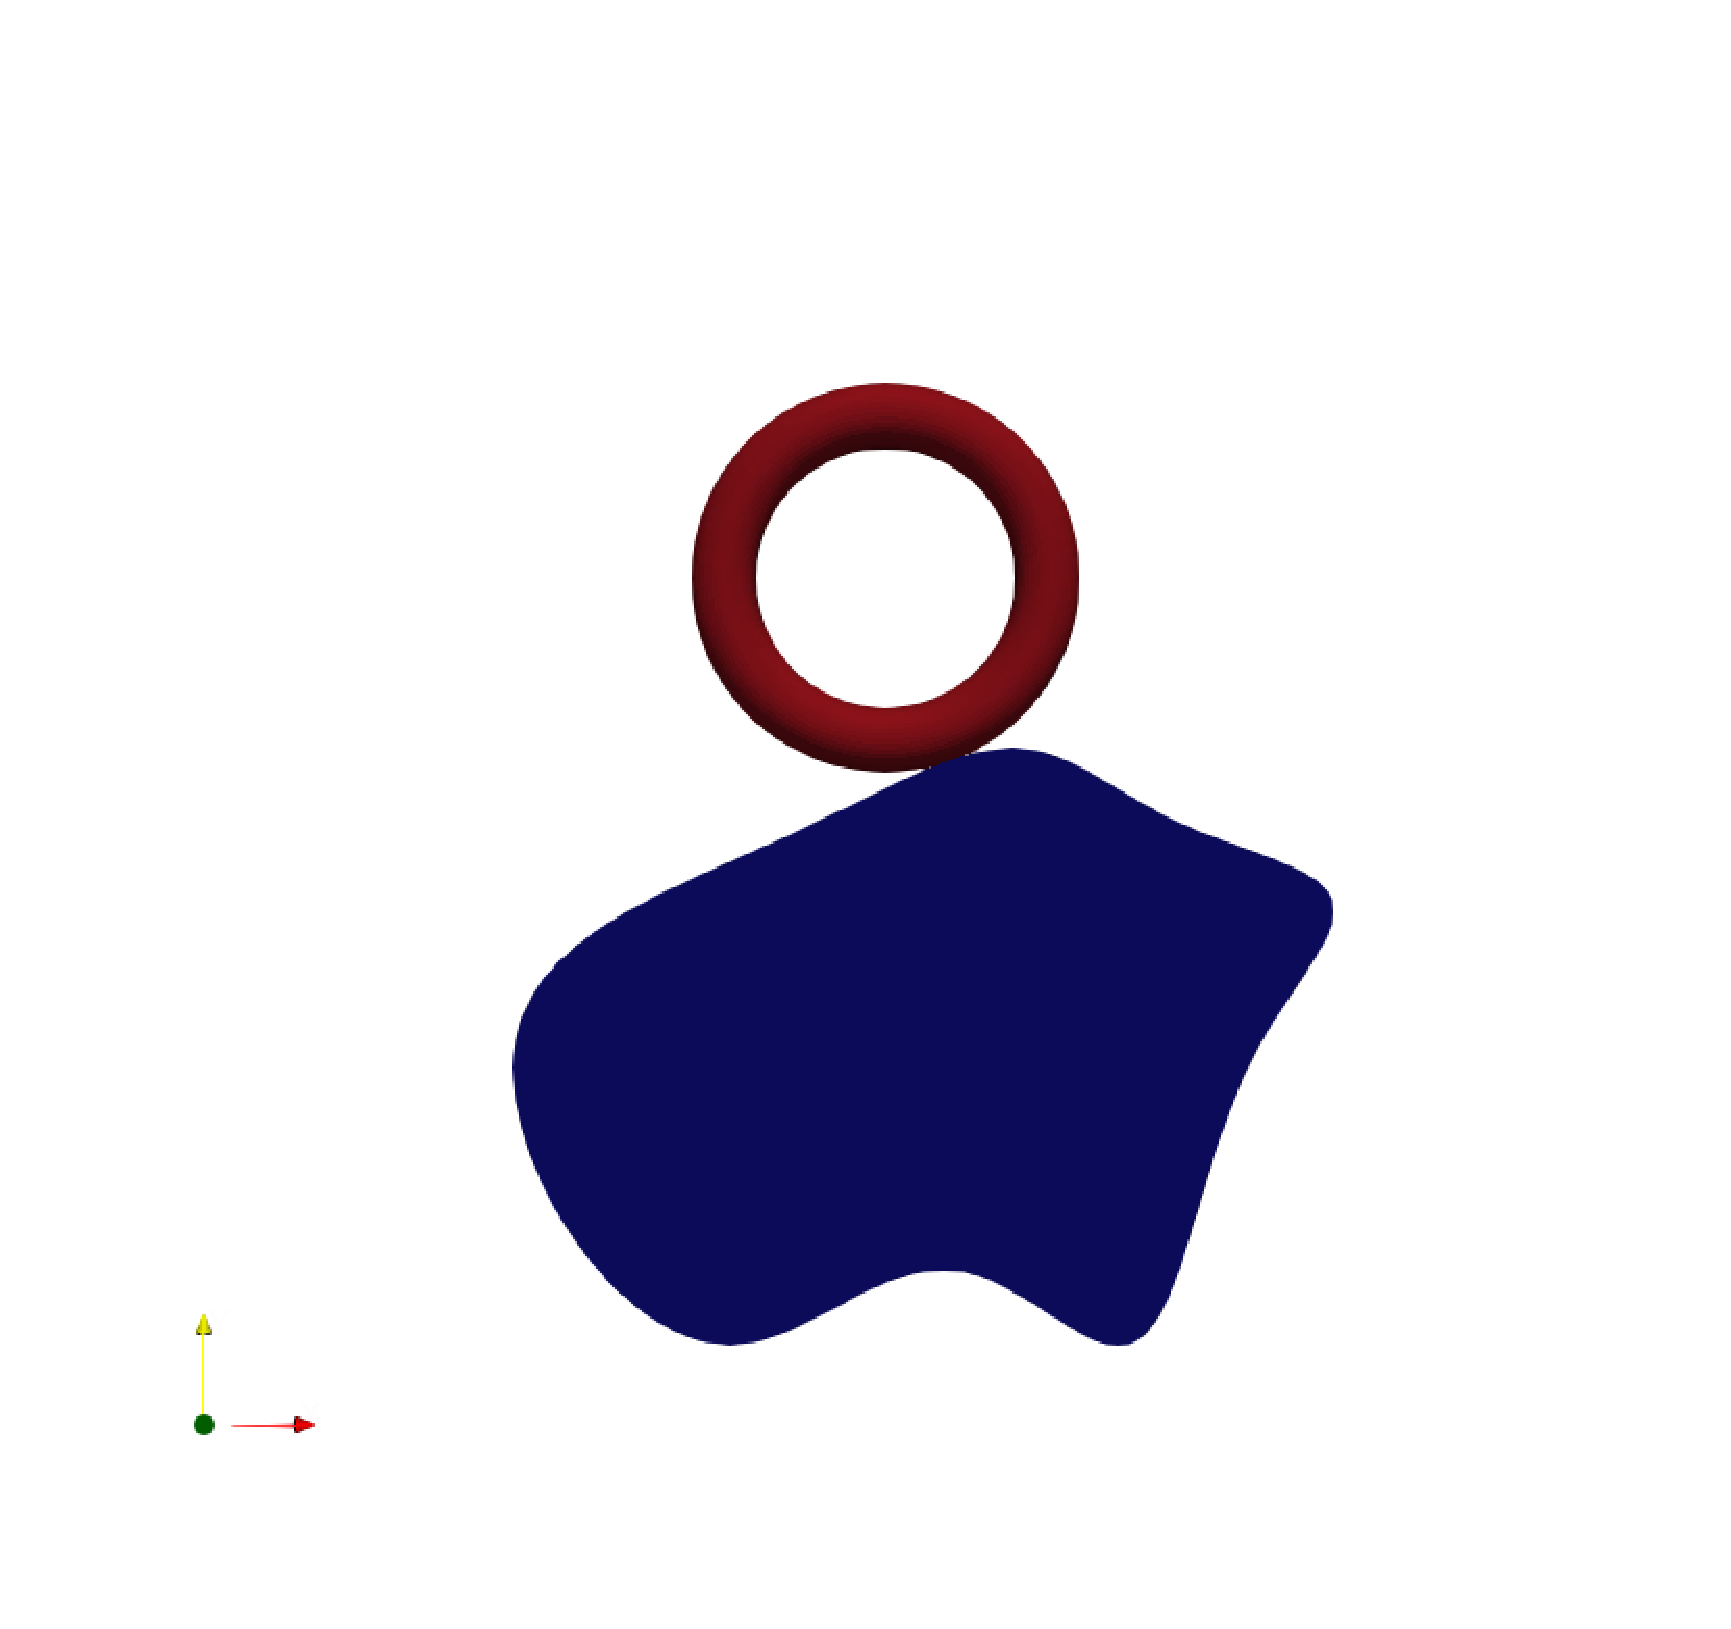
\includegraphics[width=\linewidth]{cam_1.pdf}
    \end{minipage}\hfill
    \begin{minipage}[t]{0.32\linewidth}
        \centering
        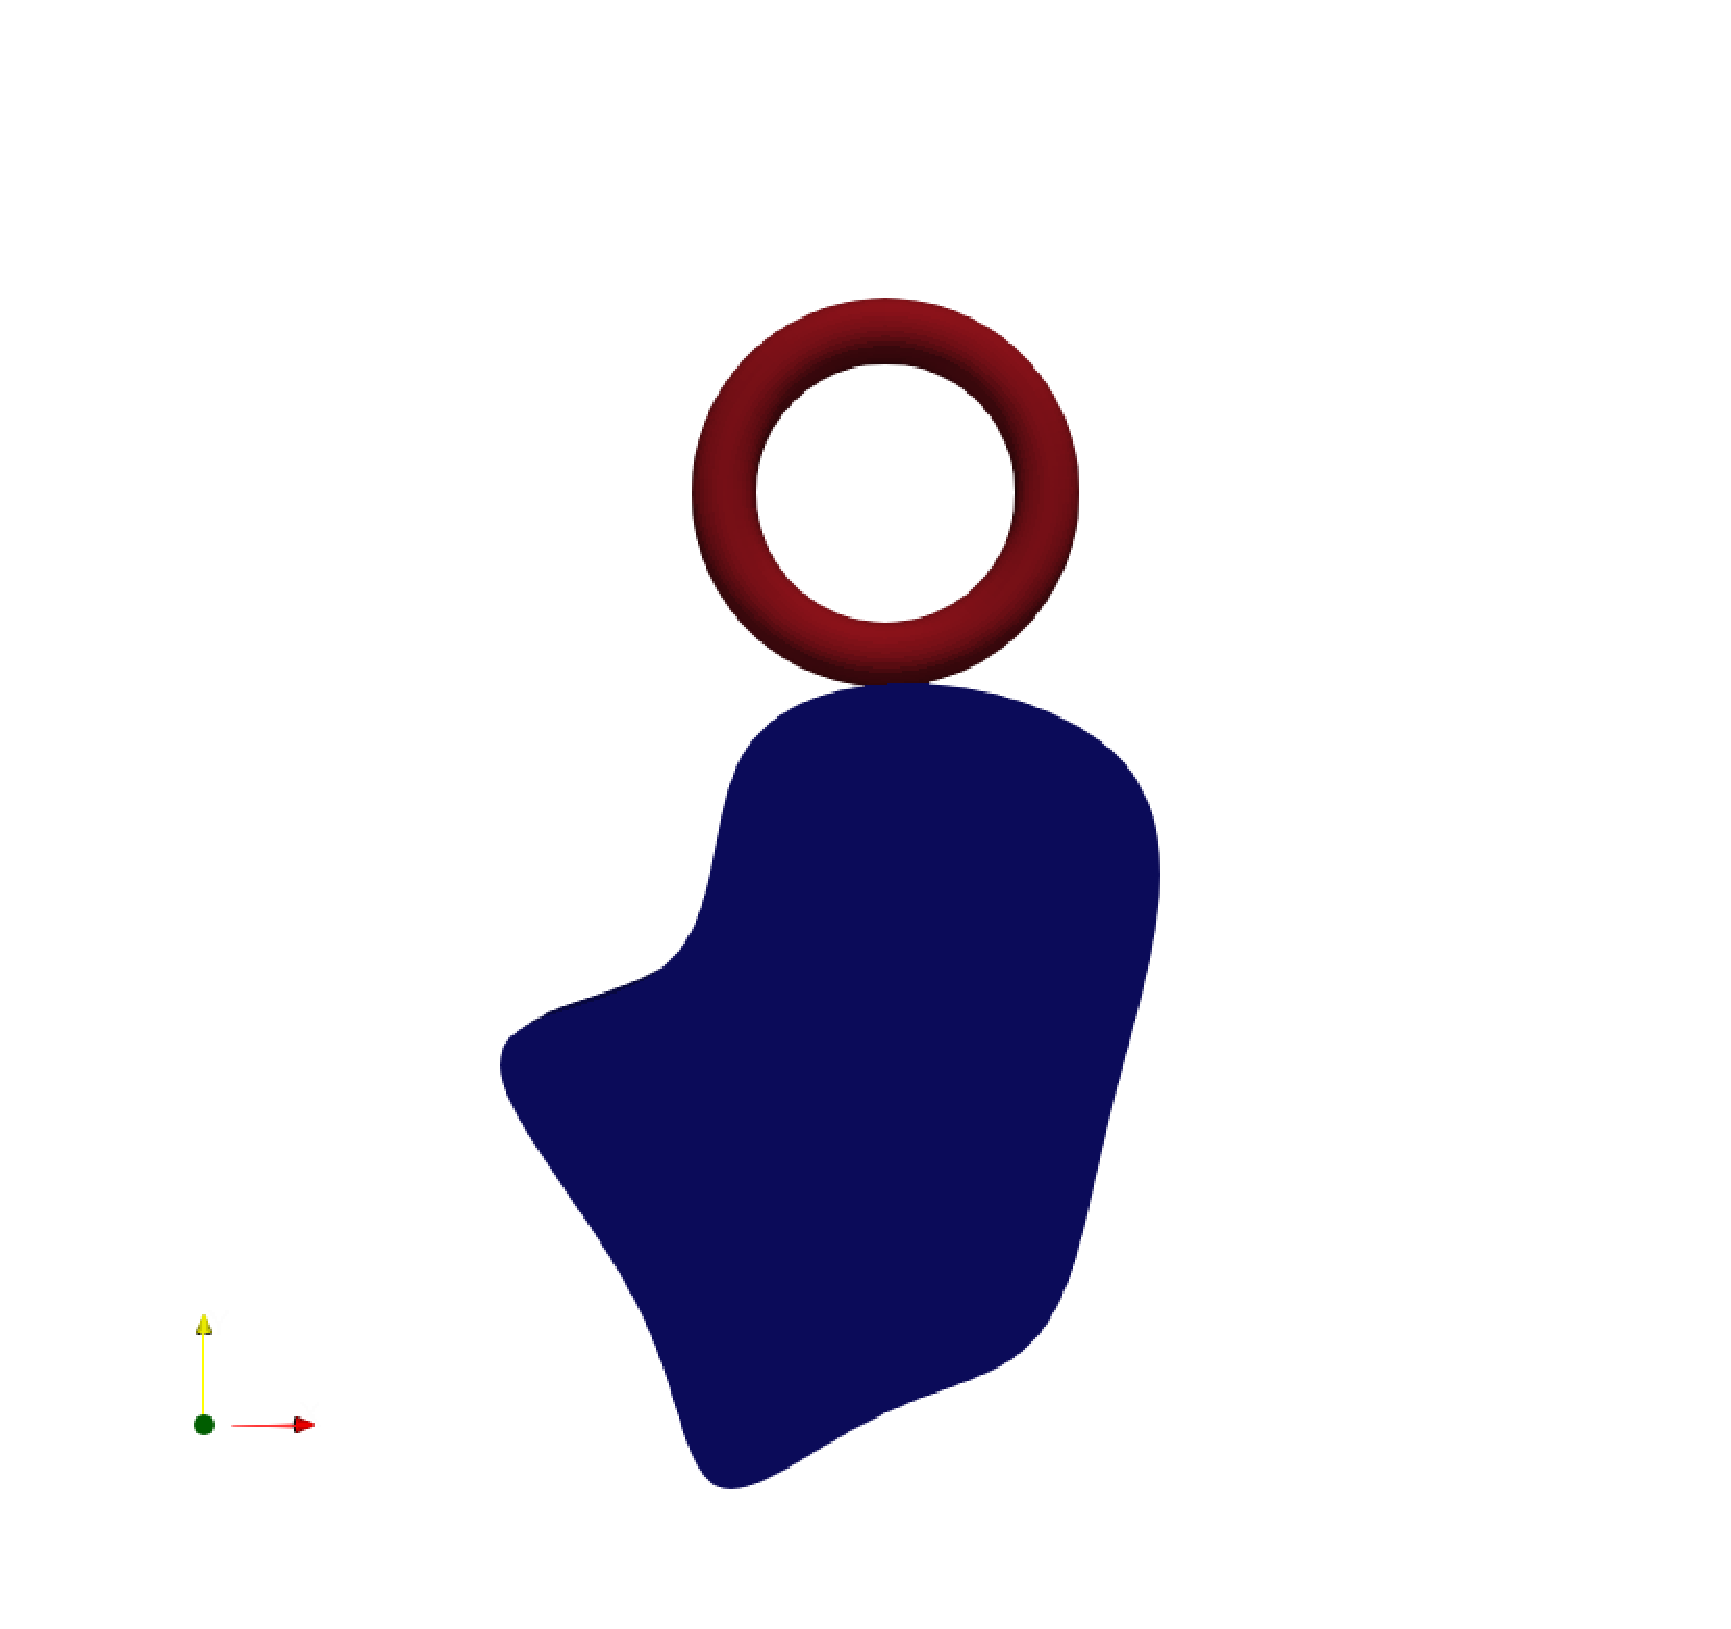
\includegraphics[width=\linewidth]{cam_2.pdf}
    \end{minipage}
    \caption{Model-state illustration of the industrial cam benchmark. From left to right: initial state, first contact, and final simulation time}
    \label{fig:cam_model}
\end{figure}

As shown in Fig. \ref{fig:accuracy}, native mesh, first-order SDF, and second-order SDF all remain stable over the full time window. The velocity RMSE is $3.4347\times 10^{-2}$ m/s for \texttt{Native Mesh}, $3.4209\times 10^{-2}$ m/s for \texttt{SdfFirstOrder}, and $3.1601\times 10^{-2}$ m/s for \texttt{SdfSecondOrder}. This indicates that, at the smaller time step, the full \texttt{SlidingPatch} path already tracks the reference curve stably, while second-order curvature feedforward still provides an additional reduction in global error.

In terms of local peaks, the SDF path also clearly outperforms native mesh. The maximum absolute velocity error of the mesh result is about $5.531\times 10^{-1}$ m/s, whereas the first- and second-order SDF results reduce it to $1.781\times 10^{-1}$ m/s and $1.725\times 10^{-1}$ m/s, respectively. This shows that under a small time step, the benefit of the second-order curvature term is not primarily a dramatic reshaping of the entire trajectory; rather, it is reflected mainly in the further suppression of a small number of locally poor windows. When local Hessian gating is consistent with the manifold-tracking strategy, second-order feedforward can yield a measurable net improvement without compromising stability.

\begin{figure}[!htbp]
    \centering
    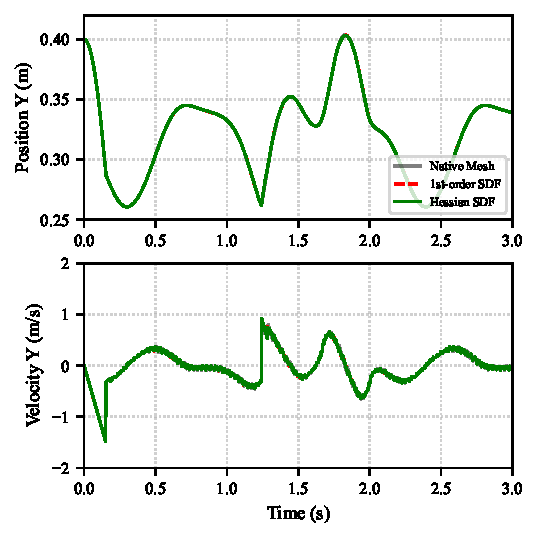
\includegraphics[width=0.94\linewidth]{fig_accuracy.pdf}
    \caption{Velocity response of the industrial cam benchmark at the base time step ($\Delta t = 0.005\text{s}$). All three solutions remain stable. The first-order SDF is comparable to the mesh result in overall RMSE but suppresses peak error more effectively, while the second-order SDF achieves the smallest overall RMSE and peak error}
    \label{fig:accuracy}
\end{figure}

\subsection{Industrial-scale performance: cam under a larger time step}
The time step of the industrial cam benchmark is then increased to $\Delta t = 0.01$ s in order to assess stability and error variation under coarser temporal resolution. Under this setting, all three methods complete the integration stably, but their accuracy levels become clearly separated:
\begin{itemize}
    \item \textbf{Native Mesh:} remains stable, but with the largest velocity error. The velocity RMSE is $5.7619\times 10^{-2}$ m/s and the maximum absolute velocity error is $7.035\times 10^{-1}$ m/s.
    \item \textbf{First-order SDF:} also remains stable and reduces the velocity RMSE to $3.3442\times 10^{-2}$ m/s, indicating that the current continuous-contact representation already supports first-order SDF solving under relatively coarse time stepping.
    \item \textbf{Second-order SDF:} further reduces the velocity RMSE to $2.4831\times 10^{-2}$ m/s while preserving stability, and yields the smallest maximum absolute velocity error of $1.572\times 10^{-1}$ m/s among the three methods.
\end{itemize}

As shown in Fig. \ref{fig:robustness}, both \texttt{SdfFirstOrder} and \texttt{SdfSecondOrder} remain stable at the larger time step and outperform native mesh overall, with second-order curvature feedforward producing the smallest global error and peak error. This indicates that as the temporal resolution becomes coarser, the advantage of the full local-geometry-aware path becomes more pronounced, and the contribution of curvature feedforward within that path also becomes more visible, providing additional accuracy gains and peak suppression. Together with the previous subsection, this suggests a clear time-step dependence of the second-order term: its benefit becomes more fully expressed under coarser time resolution.

\begin{figure}[!htbp]
    \centering
    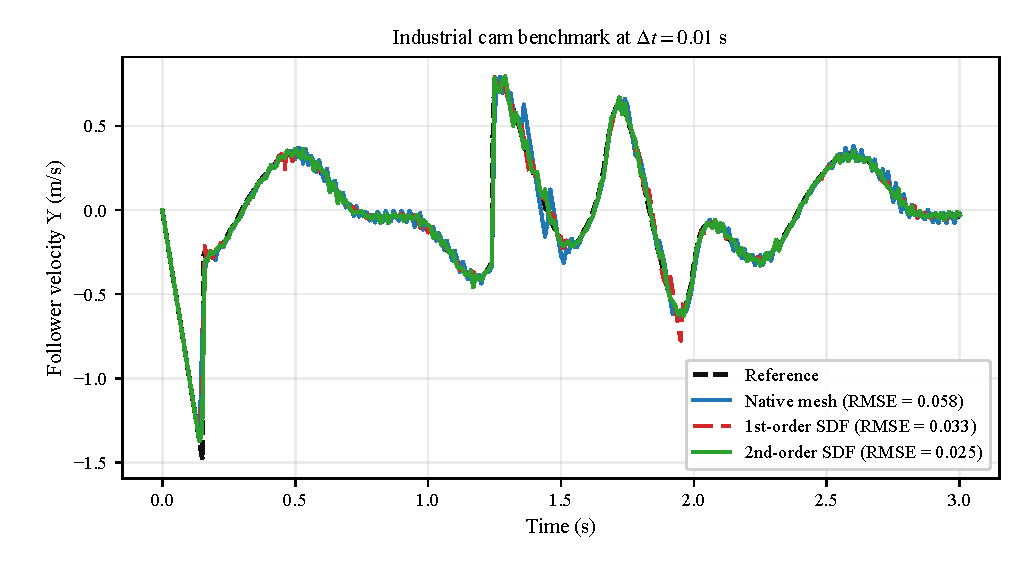
\includegraphics[width=0.94\linewidth]{fig_robustness.pdf}
    \caption{Velocity response of the industrial cam benchmark at the larger time step ($\Delta t = 0.01\text{s}$). Both SDF variants remain stable and outperform native mesh, with the second-order SDF giving the smallest velocity RMSE and peak error}
    \label{fig:robustness}
\end{figure}

\subsection{Remaining limitation: Twin Gear meshing (Twin Gear Benchmark)}
Although second-order Hessian compensation was originally designed for high-curvature contact on smooth manifolds, its performance in complex assemblies containing sharp features ($C^0$ continuity) and small backlash is equally worth separate examination. To evaluate the practical effectiveness of the method at nonsmooth boundaries, we introduce a 1:1 spur-gear meshing validation model (Twin Gear Benchmark), which simulates strongly varying multi-point contact in an extremely confined space. The mean absolute error (MAE) of the follower gear angular velocity is measured uniformly over the full time window $0 \sim 1.0$ s. The overall assembly and the local meshing region are shown in Fig. \ref{fig:twin_gear_model}.

\begin{figure}[!htbp]
    \centering
    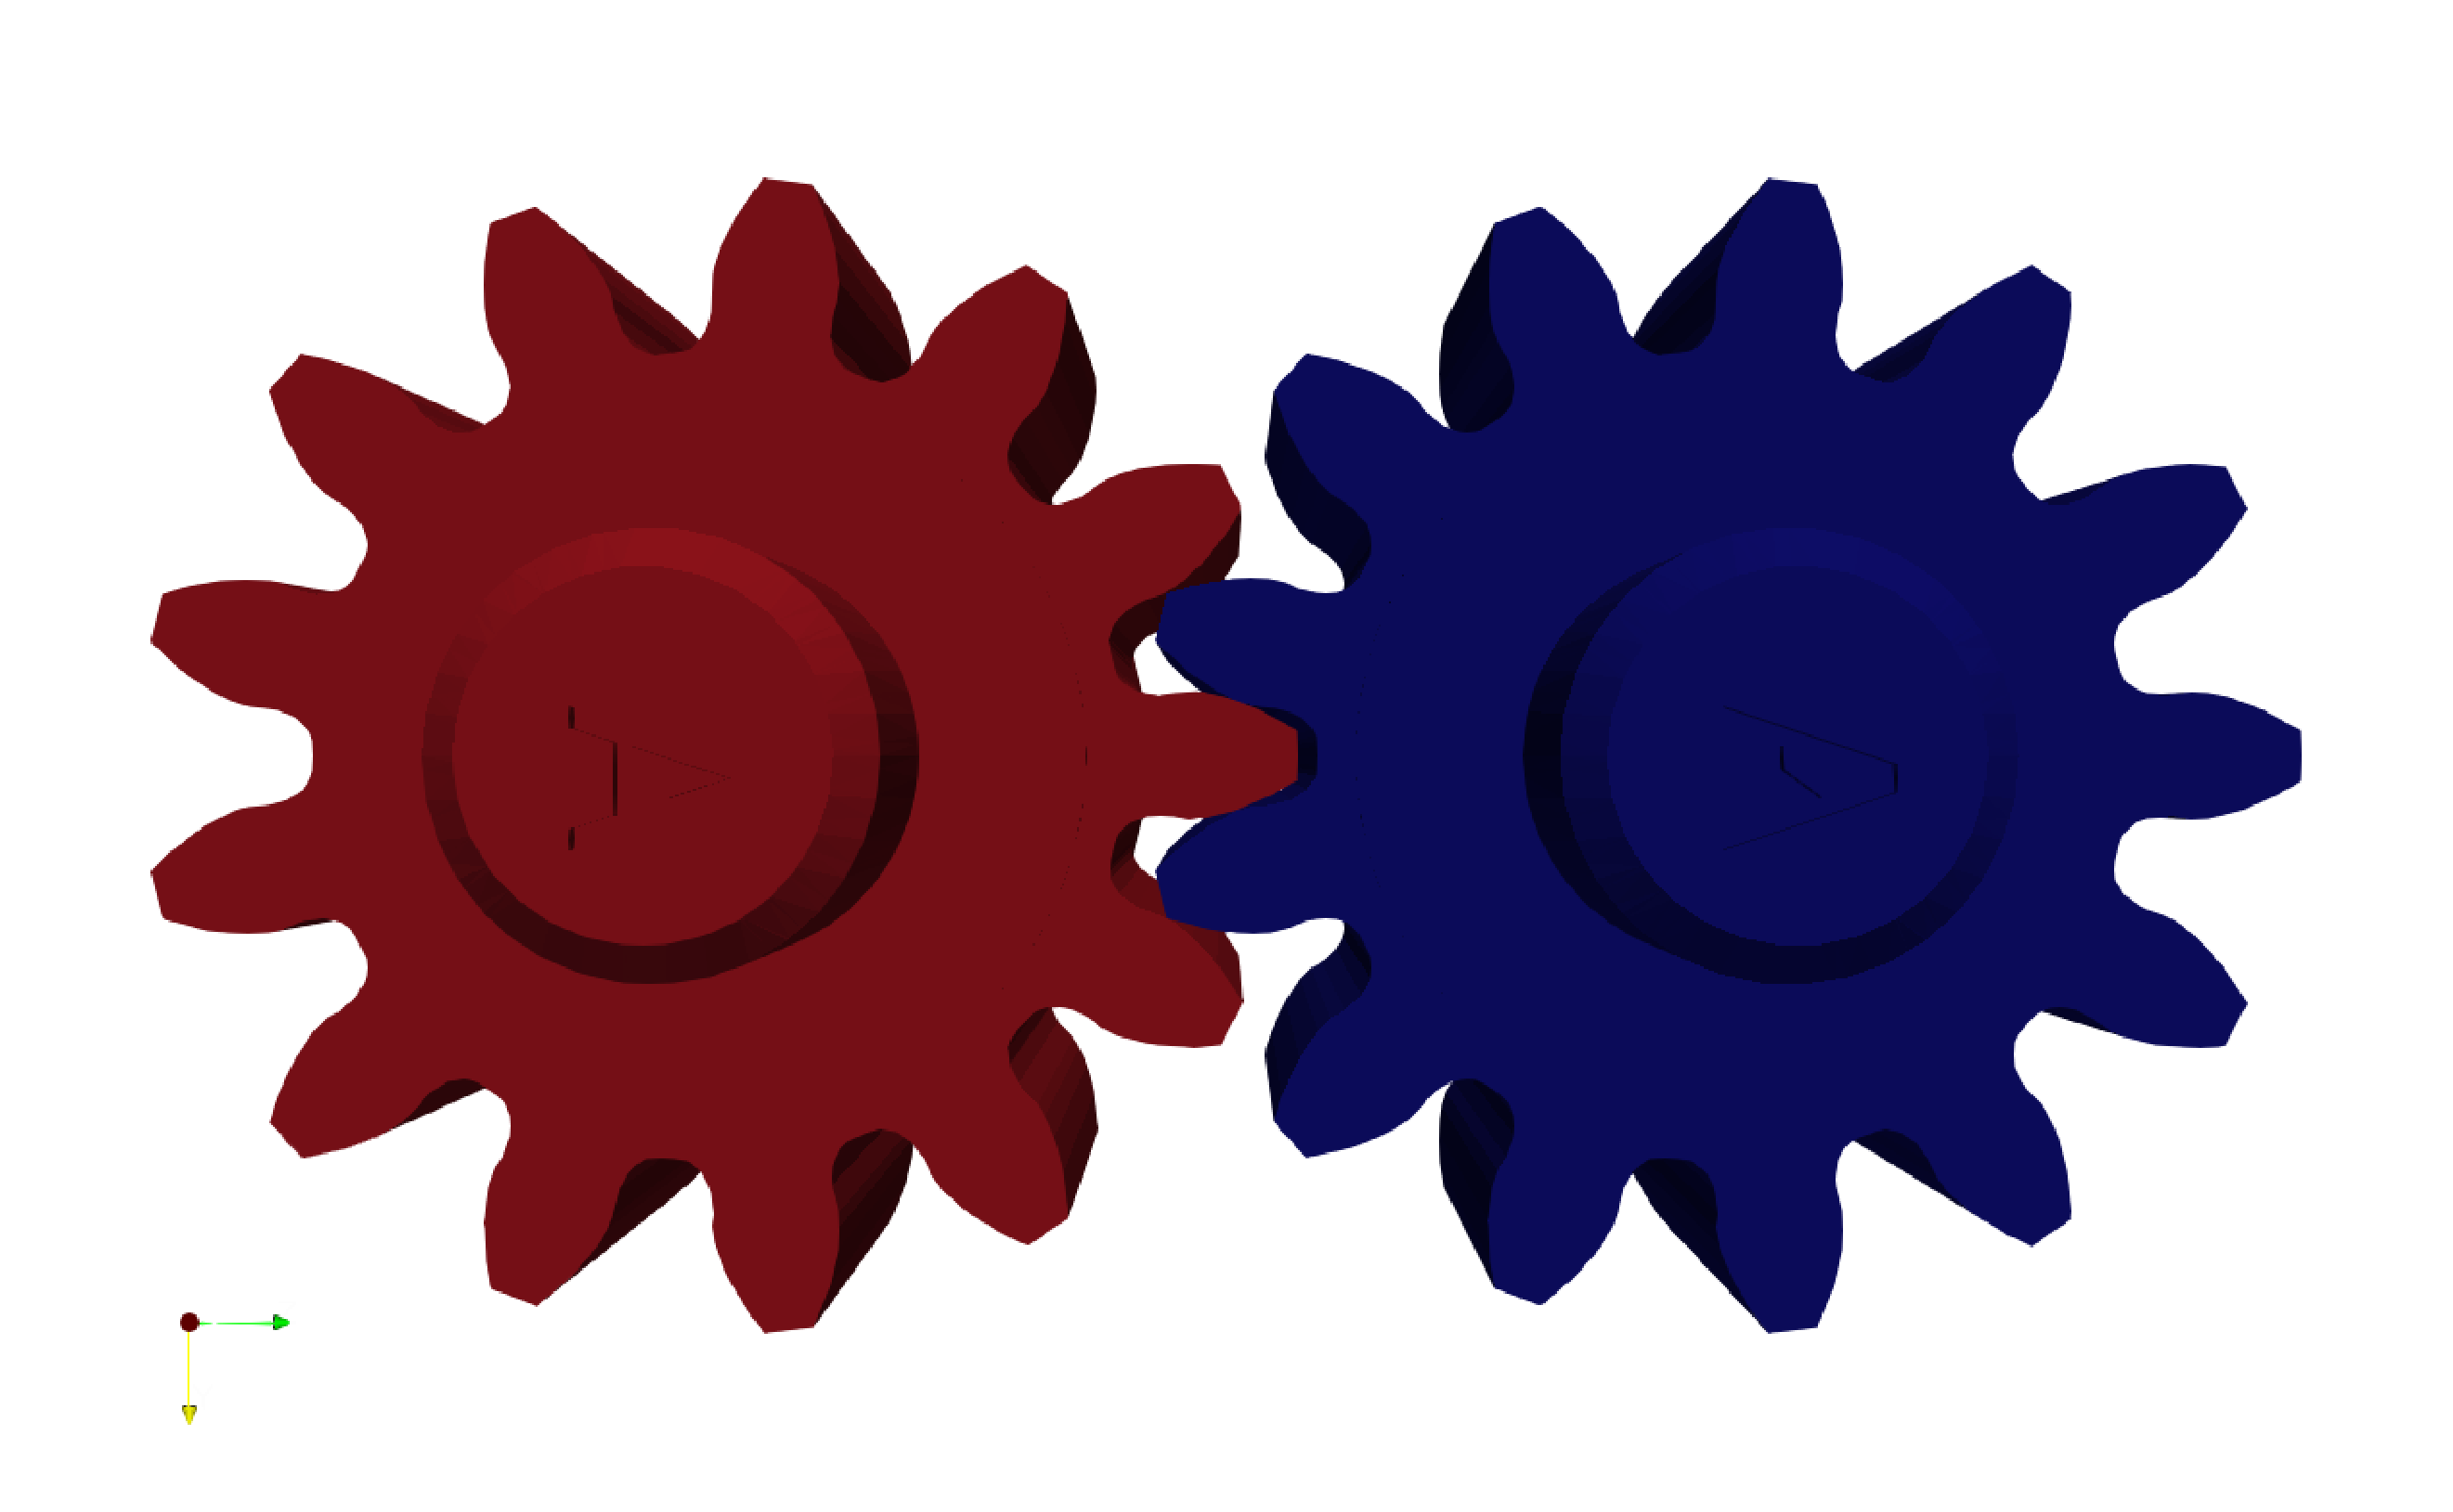
\includegraphics[height=0.35\linewidth]{gear.pdf}\hspace{0.02\linewidth}%
    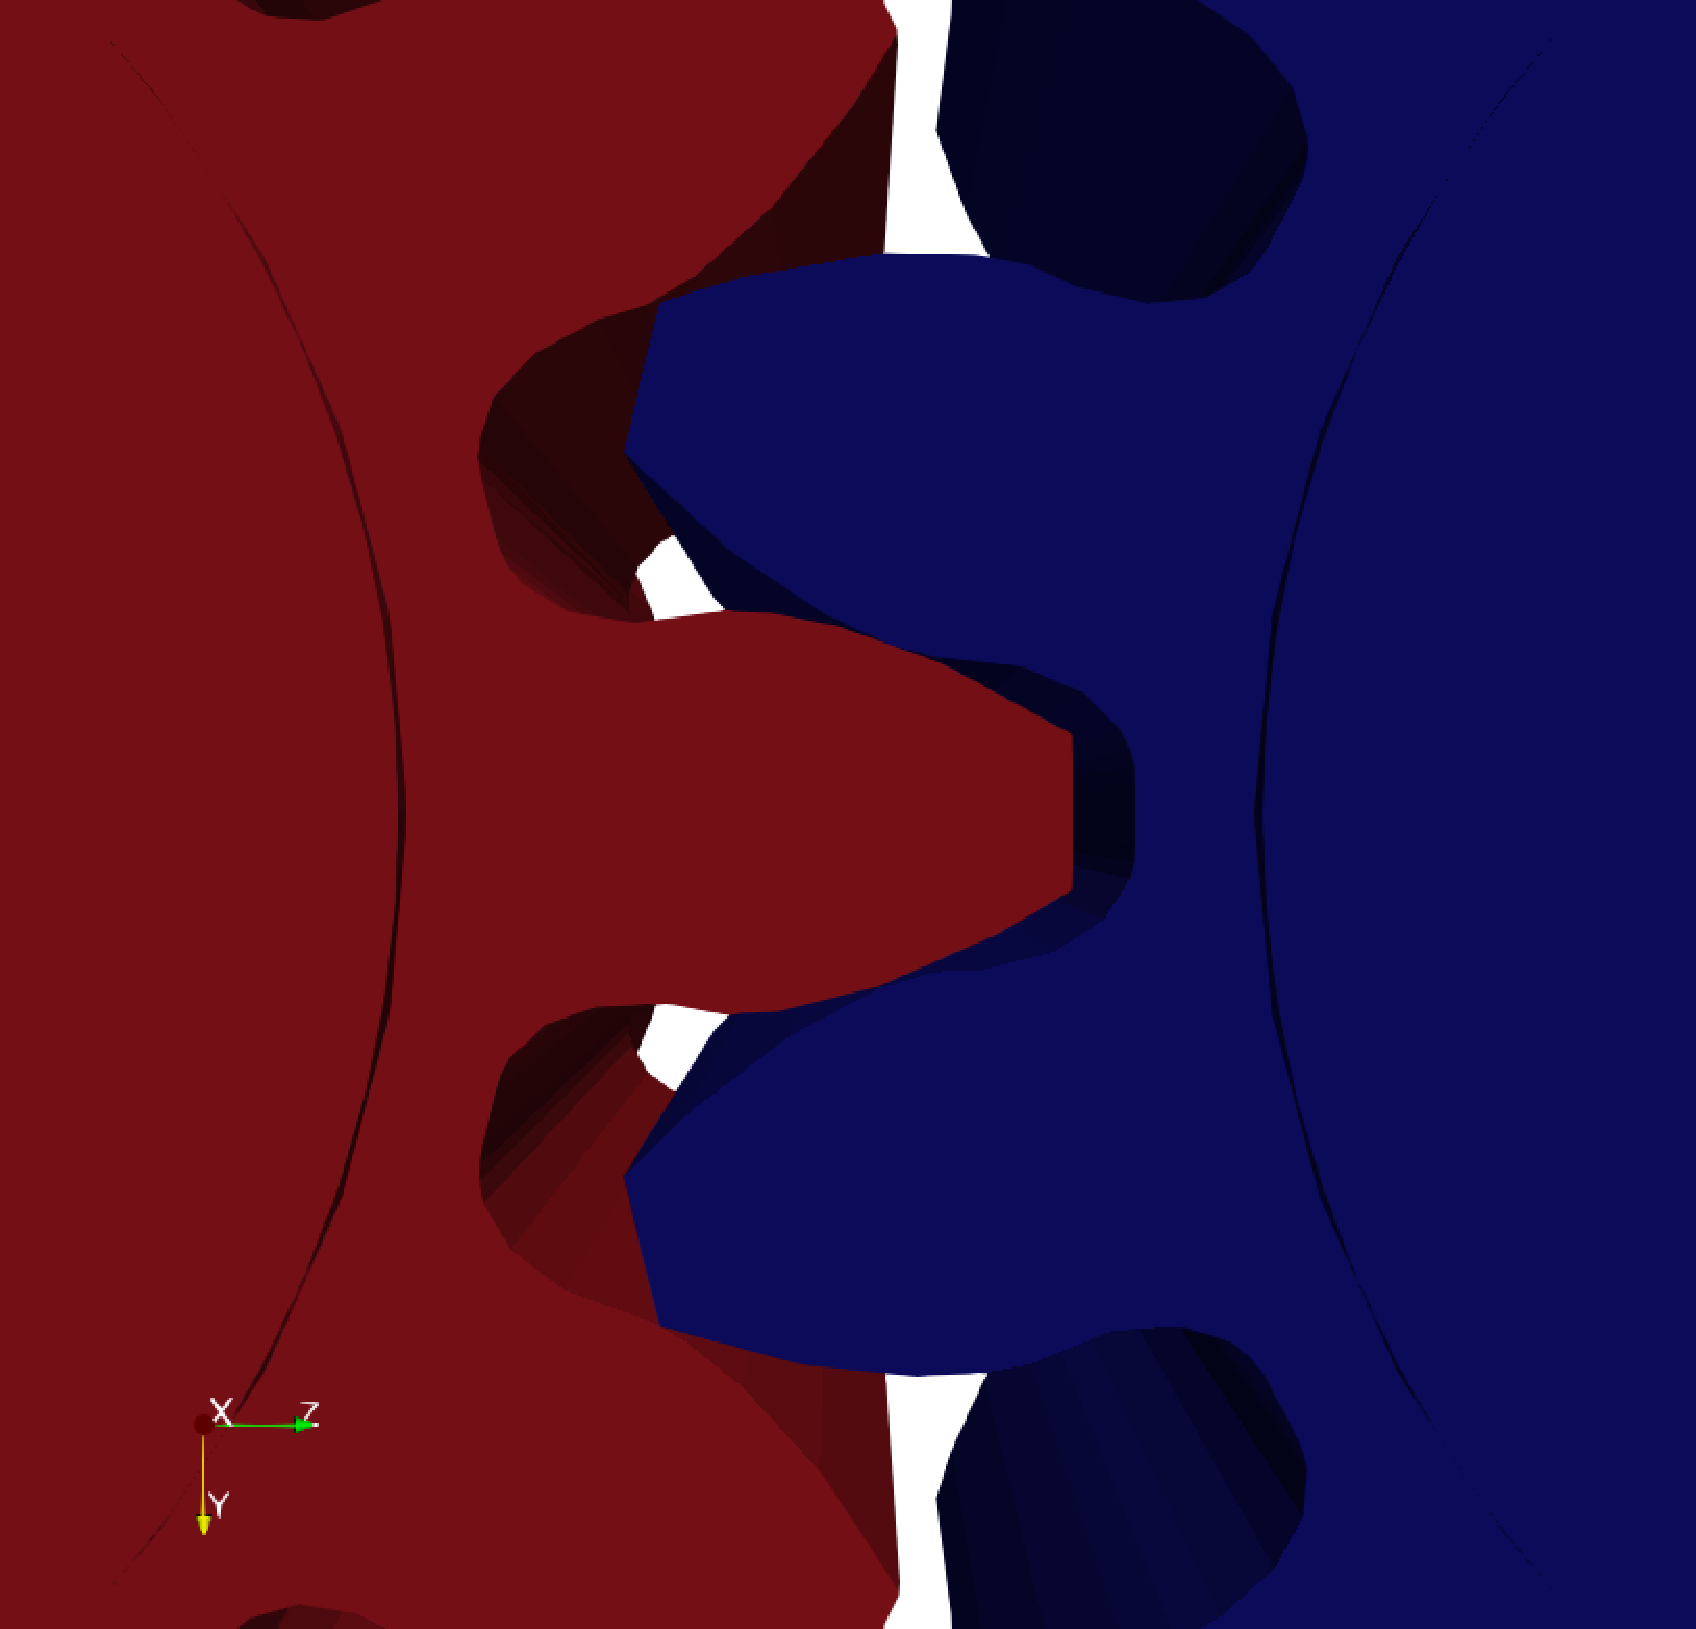
\includegraphics[height=0.35\linewidth]{gear_contact_detail.pdf}
    \caption{Model illustration of the Twin Gear benchmark. The left panel shows the overall 1:1 spur-gear assembly, and the right panel shows the local meshing region near the $C^0$ tooth-boundary transition}
    \label{fig:twin_gear_model}
\end{figure}

Under the current implementation, after introducing patch-level clustering, normal averaging, separating-velocity cutoff, and deepest-sample geometry retention, the second-order gear result no longer exhibits the early-stage degradation in which the overall error was worse than the first-order result. At a high-resolution voxel reconstruction of $20 \mu\text{m}$, the MAE of the commercial industrial baseline (Reference) is $0.0579$ rad/s; the MAE of first-order SDF is $0.0934$ rad/s; and second-order SDF further reduces it to $0.0839$ rad/s. In other words, in the current code state, second-order curvature feedforward is already able to achieve a net improvement over the first-order model in the complex gear-meshing scenario.

This improvement does not imply that the singular-geometry problem has been completely resolved. Figure \ref{fig:gear_error} shows that the second-order model indeed reduces local oscillations in the tooth-transition region and follows the global envelope more closely, but a visible gap still remains relative to the commercial industrial baseline. The reason is that at true topological singularities, such as the junction between tooth tip and tooth flank, the nearest-point branch of the signed distance field switches violently, and the dependence of the second-order curvature term on the local normal manifold remains disturbed by the nonsmooth boundary. The current patch-level manifold reduction and contact-screening strategy substantially suppress this singular feedback, but it is still insufficient to remove all residual pulses within a point-contact differential framework.

Accordingly, the current gear benchmark supports the following conclusion: \textbf{after the introduction of appropriate contact-patch reduction and geometric screening, the SDF contact path with curvature feedforward can still achieve a measurable net improvement over the first-order model even near $C^0$ singular boundaries; however, the attainable accuracy remains limited by the sensitivity of point-contact Taylor expansion to nonsmooth nearest-point branch switching.} This result shows that second-order curvature feedforward has practical value in complex assemblies, while also indicating that further progress toward industrial-grade accuracy will likely require moving beyond local point-differential formulations toward higher-dimensional integral SDF or volumetric contact representations.

\begin{figure}[!t]
    \centering
    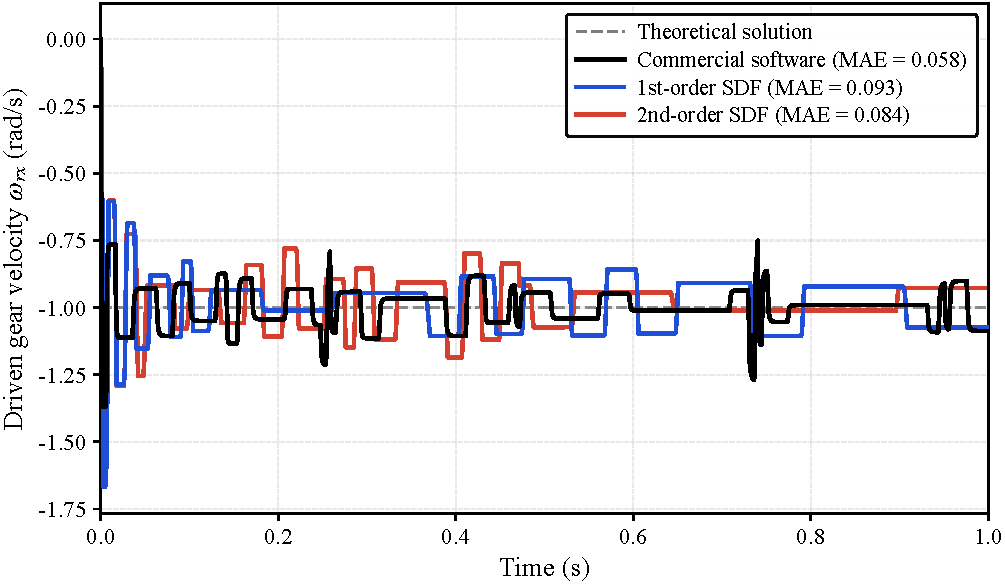
\includegraphics[width=0.94\linewidth]{gear_error.pdf}
    \caption{Transient follower-gear angular velocity response and error analysis for the Twin Gear benchmark under different curvature strategies. In the current implementation, second-order SDF improves upon first-order SDF in full-window MAE and suppresses local oscillations in the tooth-transition region, but visible residual error remains relative to the commercial industrial baseline}
    \label{fig:gear_error}
\end{figure}

\subsection{Engineering efficiency: runtime summary}
After analyzing correctness, accuracy, and limitations, we finally summarize the runtime performance of the proposed method from the standpoint of engineering deployment. Unless otherwise stated, sample-side OBB/BVH broad phase is enabled by default in the three representative continuous-sliding benchmarks considered here, namely the industrial cam, the eccentric disk--roller analytical benchmark, and the Onset Stress Benchmark, so as to reduce candidate-query cost during active-set construction. For Twin Gear, it remains disabled by default and is used only in offline comparisons to verify losslessness and benefit boundaries. This setting reflects a basic principle of the present work: hierarchical broad phase must also be matched to the preset regime and the associated local manifold shape, rather than being uniformly forced on all benchmarks.

For practical deployment in engineering-scale complex assembly simulation, the additional algorithmic overhead is critical because both explicit and implicit multibody stepping are subject to strict runtime constraints. In the current implementation, native mesh contact still relies on an explicit mesh-geometry contact chain, whereas the SDF path reuses the same LCP solution backbone and adds sample-side OBB/BVH broad phase only in continuous-sliding benchmarks. Tables \ref{tab:runtime_overview} and \ref{tab:error_overview} therefore report the formal runtime and main error metrics for three representative continuous-contact benchmarks.

These data show that the extra cost of second-order curvature feedforward does not push the SDF path back into the runtime range of native mesh contact. On the contrary, in the current implementation state, \texttt{SdfSecondOrder} remains on the same order of computational cost as \texttt{SdfFirstOrder} for the industrial cam, eccentric disk--roller, and Onset Stress benchmarks, while delivering consistent net gains in accuracy. For these representative continuous-contact benchmarks, the evidence therefore supports the central claim of this paper: under regime-matched local representations, improved contact-response accuracy can be obtained while keeping computational cost low. The present local-geometry-aware modeling strategy is therefore not simply a matter of ``more expensive contact solving,'' but a way of making efficiency and accuracy coexist through matched local manifold representations and hierarchical candidate detection.

\begin{table}[htbp]
    \centering
    \caption{Total runtime comparison for representative continuous-contact benchmarks}
    \label{tab:runtime_overview}
    \resizebox{\columnwidth}{!}{
    \begin{tabular}{lccc}
        \toprule
        \textbf{Benchmark} & \textbf{Native Mesh} & \textbf{SDF 1st-order} & \textbf{SDF 2nd-order} \\
        \midrule
        Industrial cam ($\Delta t=0.01$ s, $T=3.0$ s) & $135.9$ s & $15.0$ s & $16.0$ s \\
        Eccentric disk--roller ($\Delta t=0.002$ s, $T=\pi/2$ s) & $149.4$ s & $2.07$ s & $2.23$ s \\
        Onset Stress B ($\Delta t=0.001$ s) & $111.5$ s & $35.4$ s & $36.4$ s \\
        \bottomrule
    \end{tabular}
    }
\end{table}

\begin{table}[htbp]
    \centering
    \caption{Main error metrics for representative continuous-contact benchmarks}
    \label{tab:error_overview}
    \resizebox{\columnwidth}{!}{
    \begin{tabular}{lccc}
        \toprule
        \textbf{Benchmark} & \textbf{Native Mesh} & \textbf{SDF 1st-order} & \textbf{SDF 2nd-order} \\
        \midrule
        Industrial cam (velocity RMSE) & $0.0576$ & $0.0334$ & $0.0248$ \\
        Eccentric disk--roller (velocity RMSE) & $9.27\times10^{-4}$ & $6.94\times10^{-4}$ & $6.88\times10^{-4}$ \\
        Onset Stress B (velocity RMSE) & $8.59\times10^{-4}$ & $8.43\times10^{-4}$ & $8.41\times10^{-4}$ \\
        \bottomrule
    \end{tabular}
    }
\end{table}


\section{Conclusion}
This paper has proposed and validated a \textbf{local-geometry-aware contact modeling strategy} for complementarity-based rigid contact. Within an existing hard-contact solution framework, local SDF information is used to construct contact representations near the active region, while \texttt{SlidingPatch} and \texttt{CompactDiscrete} are selected according to the contact state. The method does not replace the underlying time-stepping or LCP solution chain; instead, it strengthens local geometric representation at the contact-modeling level. The regime choice is always preset at the case or application level. The reported results therefore support a modeling principle rather than a runtime automatic regime-identification algorithm.

The numerical results show that local geometry awareness is effective within the intended scope of complementarity-based rigid contact, but that its benefit is strongly state-dependent. For sustained sliding with relatively smooth local geometry, continuous patch representations make fuller use of local geometric information and improve trajectory and velocity responses while keeping the additional modeling cost modest, thereby preserving computational efficiency and improving contact-response accuracy at the same time. For contact onset, state transitions, and locally singular configurations, more compact and conservative discrete representations provide better robustness. The continuous-contact benchmarks therefore validate the full local-geometry-aware modeling stack, whereas the difference between first- and second-order SDF isolates the incremental contribution of curvature feedforward. The industrial cam, analytical roller, and Onset Stress cases support this interpretation, while the Twin Gear benchmark shows that a structural error floor remains in nonsmooth meshing with violent branch switching.

The main conclusion can therefore be stated as follows: \textbf{within the intended application range of complementarity-based rigid contact, a regime-matched local geometric representation can maintain computational efficiency while achieving more accurate contact responses without modifying the underlying solution chain.} Geometry awareness becomes a stable and useful numerical ingredient only when the representation is coordinated with the contact state. The present results do not support a claim of universal optimality for any single regime. They instead support a modeling principle in which local representations are configured according to contact state under clearly stated applicability conditions and failure boundaries. This conclusion provides a clearer basis for the construction, comparison, and engineering deployment of future complementarity-based rigid-contact models.

From a modeling perspective, these results indicate that, even when the underlying LCP solution chain is left unchanged, substantial room for improvement remains at the geometry-input layer of rigid-contact computation. In cases where response error is dominated by gap-prediction bias, distortion of the local normal manifold, and noise during contact activation, the way local geometric information enters the contact model directly affects final accuracy. The present contribution is therefore better understood as a geometric-modeling reinforcement of an established complementarity-based rigid-contact pipeline: its main role is not to replace the underlying solution theory, but to improve the quality of the existing modeling interface through low-intrusion local geometric representations.

Although the present method has been validated only for complementarity-based rigid contact, the current results already indicate that the local geometric and differential information encoded by the SDF can serve as an effective auxiliary quantity in contact computation, improving numerical response under clearly defined applicability conditions and indicating that computational efficiency and response accuracy can coexist within the intended application regimes. In this sense, local geometry awareness should not be viewed solely as a case-specific refinement within the current rigid-body framework, but may point toward a broader modeling direction for contact computation. Future work will therefore examine how richer local spatial geometric descriptors can be incorporated systematically into contact computation for flexible-body contact and for broader classes of contact solvers.


\section*{Statements and Declarations}
\textbf{Funding} The authors received no external funding for this study.

\textbf{Competing interests} The authors declare that they have no competing interests.

\textbf{Data availability} The datasets generated or analyzed during the current study are not publicly available because they include project-specific geometric models, benchmark configurations, and implementation-dependent simulation outputs. They are available from the corresponding author on reasonable request for academic research use.

\textbf{Code availability} The research code is part of an actively developed in-house simulation framework and is therefore not publicly released at this stage. A research-use version of the implementation can be made available from the corresponding author on reasonable request, subject to project-specific licensing and redistribution constraints.


\bibliographystyle{plainurl}
\bibliography{../references,../references_extra}

\end{document}
